\documentclass[twoside]{book}

% Packages required by doxygen
\usepackage{calc}
\usepackage{doxygen}
\usepackage{graphicx}
\usepackage[utf8]{inputenc}
\usepackage{makeidx}
\usepackage{multicol}
\usepackage{multirow}
\usepackage{textcomp}
\usepackage[table]{xcolor}

% Font selection
\usepackage[T1]{fontenc}
\usepackage{mathptmx}
\usepackage[scaled=.90]{helvet}
\usepackage{courier}
\usepackage{amssymb}
\usepackage{sectsty}
\renewcommand{\familydefault}{\sfdefault}
\allsectionsfont{%
  \fontseries{bc}\selectfont%
  \color{darkgray}%
}
\renewcommand{\DoxyLabelFont}{%
  \fontseries{bc}\selectfont%
  \color{darkgray}%
}

% Page & text layout
\usepackage{geometry}
\geometry{%
  a4paper,%
  top=2.5cm,%
  bottom=2.5cm,%
  left=2.5cm,%
  right=2.5cm%
}
\tolerance=750
\hfuzz=15pt
\hbadness=750
\setlength{\emergencystretch}{15pt}
\setlength{\parindent}{0cm}
\setlength{\parskip}{0.2cm}
\makeatletter
\renewcommand{\paragraph}{%
  \@startsection{paragraph}{4}{0ex}{-1.0ex}{1.0ex}{%
    \normalfont\normalsize\bfseries\SS@parafont%
  }%
}
\renewcommand{\subparagraph}{%
  \@startsection{subparagraph}{5}{0ex}{-1.0ex}{1.0ex}{%
    \normalfont\normalsize\bfseries\SS@subparafont%
  }%
}
\makeatother

% Headers & footers
\usepackage{fancyhdr}
\pagestyle{fancyplain}
\fancyhead[LE]{\fancyplain{}{\bfseries\thepage}}
\fancyhead[CE]{\fancyplain{}{}}
\fancyhead[RE]{\fancyplain{}{\bfseries\leftmark}}
\fancyhead[LO]{\fancyplain{}{\bfseries\rightmark}}
\fancyhead[CO]{\fancyplain{}{}}
\fancyhead[RO]{\fancyplain{}{\bfseries\thepage}}
\fancyfoot[LE]{\fancyplain{}{}}
\fancyfoot[CE]{\fancyplain{}{}}
\fancyfoot[RE]{\fancyplain{}{\bfseries\scriptsize Generated on Tue Feb 16 2016 02\-:38\-:37 by Doxygen }}
\fancyfoot[LO]{\fancyplain{}{\bfseries\scriptsize Generated on Tue Feb 16 2016 02\-:38\-:37 by Doxygen }}
\fancyfoot[CO]{\fancyplain{}{}}
\fancyfoot[RO]{\fancyplain{}{}}
\renewcommand{\footrulewidth}{0.4pt}
\renewcommand{\chaptermark}[1]{%
  \markboth{#1}{}%
}
\renewcommand{\sectionmark}[1]{%
  \markright{\thesection\ #1}%
}

% Indices & bibliography
\usepackage{natbib}
\usepackage[titles]{tocloft}
\setcounter{tocdepth}{3}
\setcounter{secnumdepth}{5}
\makeindex

% Hyperlinks (required, but should be loaded last)
\usepackage{ifpdf}
\ifpdf
  \usepackage[pdftex,pagebackref=true]{hyperref}
\else
  \usepackage[ps2pdf,pagebackref=true]{hyperref}
\fi
\hypersetup{%
  colorlinks=true,%
  linkcolor=blue,%
  citecolor=blue,%
  unicode%
}

% Custom commands
\newcommand{\clearemptydoublepage}{%
  \newpage{\pagestyle{empty}\cleardoublepage}%
}


%===== C O N T E N T S =====

\begin{document}

% Titlepage & ToC
\hypersetup{pageanchor=false}
\pagenumbering{roman}
\begin{titlepage}
\vspace*{7cm}
\begin{center}%
{\Large Reference Manual}\\
\vspace*{1cm}
{\large Generated by Doxygen 1.8.6}\\
\vspace*{0.5cm}
{\small Tue Feb 16 2016 02:38:37}\\
\end{center}
\end{titlepage}
\clearemptydoublepage
\tableofcontents
\clearemptydoublepage
\pagenumbering{arabic}
\hypersetup{pageanchor=true}

%--- Begin generated contents ---
\chapter{Hierarchical Index}
\section{Class Hierarchy}
This inheritance list is sorted roughly, but not completely, alphabetically\-:\begin{DoxyCompactList}
\item \contentsline{section}{fuse.\-Logging\-Mix\-In}{\pageref{classfuse_1_1LoggingMixIn}}{}
\item object\begin{DoxyCompactList}
\item \contentsline{section}{fuse.\-F\-U\-S\-E}{\pageref{classfuse_1_1FUSE}}{}
\item \contentsline{section}{fuse.\-Operations}{\pageref{classfuse_1_1Operations}}{}
\begin{DoxyCompactList}
\item \contentsline{section}{nfio.\-Nfio}{\pageref{classnfio_1_1Nfio}}{}
\end{DoxyCompactList}
\item \contentsline{section}{hypervisor.\-hypervisor\-\_\-base.\-Hypervisor\-Base}{\pageref{classhypervisor_1_1hypervisor__base_1_1HypervisorBase}}{}
\item \contentsline{section}{hypervisor.\-hypervisor\-\_\-factory.\-Hypervisor\-Factory}{\pageref{classhypervisor_1_1hypervisor__factory_1_1HypervisorFactory}}{}
\end{DoxyCompactList}
\item O\-S\-Error\begin{DoxyCompactList}
\item \contentsline{section}{fuse.\-Fuse\-O\-S\-Error}{\pageref{classfuse_1_1FuseOSError}}{}
\end{DoxyCompactList}
\item Structure\begin{DoxyCompactList}
\item \contentsline{section}{fuse.\-c\-\_\-stat}{\pageref{classfuse_1_1c__stat}}{}
\item \contentsline{section}{fuse.\-c\-\_\-statvfs}{\pageref{classfuse_1_1c__statvfs}}{}
\item \contentsline{section}{fuse.\-c\-\_\-statvfs}{\pageref{classfuse_1_1c__statvfs}}{}
\item \contentsline{section}{fuse.\-c\-\_\-timespec}{\pageref{classfuse_1_1c__timespec}}{}
\item \contentsline{section}{fuse.\-c\-\_\-utimbuf}{\pageref{classfuse_1_1c__utimbuf}}{}
\item \contentsline{section}{fuse.\-fuse\-\_\-context}{\pageref{classfuse_1_1fuse__context}}{}
\item \contentsline{section}{fuse.\-fuse\-\_\-file\-\_\-info}{\pageref{classfuse_1_1fuse__file__info}}{}
\item \contentsline{section}{fuse.\-fuse\-\_\-operations}{\pageref{classfuse_1_1fuse__operations}}{}
\end{DoxyCompactList}
\item \contentsline{section}{vnfs\-\_\-operations.\-V\-N\-F\-S\-Operations}{\pageref{classvnfs__operations_1_1VNFSOperations}}{}
\item Hypervisor\-Base\begin{DoxyCompactList}
\item \contentsline{section}{hypervisor.\-docker\-\_\-driver.\-Docker}{\pageref{classhypervisor_1_1docker__driver_1_1Docker}}{}
\item \contentsline{section}{hypervisor.\-libvirt\-\_\-driver.\-Libvirt}{\pageref{classhypervisor_1_1libvirt__driver_1_1Libvirt}}{}
\end{DoxyCompactList}
\end{DoxyCompactList}

\chapter{Class Index}
\section{Class List}
Here are the classes, structs, unions and interfaces with brief descriptions\-:\begin{DoxyCompactList}
\item\contentsline{section}{\hyperlink{classhypervisor_1_1docker__driver_1_1DockerDriver}{hypervisor.\-docker\-\_\-driver.\-Docker\-Driver} \\*Docker driver for nfio }{\pageref{classhypervisor_1_1docker__driver_1_1DockerDriver}}{}
\item\contentsline{section}{\hyperlink{classhypervisor_1_1hypervisor__base_1_1HypervisorBase}{hypervisor.\-hypervisor\-\_\-base.\-Hypervisor\-Base} \\*Base class for hypervisors }{\pageref{classhypervisor_1_1hypervisor__base_1_1HypervisorBase}}{}
\item\contentsline{section}{\hyperlink{classerrors_1_1HypervisorConnectionError}{errors.\-Hypervisor\-Connection\-Error} }{\pageref{classerrors_1_1HypervisorConnectionError}}{}
\item\contentsline{section}{\hyperlink{classerrors_1_1HypervisorError}{errors.\-Hypervisor\-Error} }{\pageref{classerrors_1_1HypervisorError}}{}
\item\contentsline{section}{\hyperlink{classhypervisor_1_1hypervisor__factory_1_1HypervisorFactory}{hypervisor.\-hypervisor\-\_\-factory.\-Hypervisor\-Factory} \\*A singletone class for creating hypervisor driver objects }{\pageref{classhypervisor_1_1hypervisor__factory_1_1HypervisorFactory}}{}
\item\contentsline{section}{\hyperlink{classhypervisor_1_1libvirt__driver_1_1Libvirt}{hypervisor.\-libvirt\-\_\-driver.\-Libvirt} }{\pageref{classhypervisor_1_1libvirt__driver_1_1Libvirt}}{}
\item\contentsline{section}{\hyperlink{classnfio_1_1Nfio}{nfio.\-Nfio} }{\pageref{classnfio_1_1Nfio}}{}
\item\contentsline{section}{\hyperlink{classerrors_1_1nfioError}{errors.\-nfio\-Error} \\*This module contains all the custom exceptions defined for nf.\-io }{\pageref{classerrors_1_1nfioError}}{}
\item\contentsline{section}{\hyperlink{classerrors_1_1VNFCommandExecutionError}{errors.\-V\-N\-F\-Command\-Execution\-Error} }{\pageref{classerrors_1_1VNFCommandExecutionError}}{}
\item\contentsline{section}{\hyperlink{classerrors_1_1VNFConfigurationError}{errors.\-V\-N\-F\-Configuration\-Error} }{\pageref{classerrors_1_1VNFConfigurationError}}{}
\item\contentsline{section}{\hyperlink{classerrors_1_1VNFCreateError}{errors.\-V\-N\-F\-Create\-Error} }{\pageref{classerrors_1_1VNFCreateError}}{}
\item\contentsline{section}{\hyperlink{classerrors_1_1VNFDeployError}{errors.\-V\-N\-F\-Deploy\-Error} }{\pageref{classerrors_1_1VNFDeployError}}{}
\item\contentsline{section}{\hyperlink{classerrors_1_1VNFDeployErrorWithInconsistentState}{errors.\-V\-N\-F\-Deploy\-Error\-With\-Inconsistent\-State} }{\pageref{classerrors_1_1VNFDeployErrorWithInconsistentState}}{}
\item\contentsline{section}{\hyperlink{classerrors_1_1VNFDestroyError}{errors.\-V\-N\-F\-Destroy\-Error} }{\pageref{classerrors_1_1VNFDestroyError}}{}
\item\contentsline{section}{\hyperlink{classerrors_1_1VNFHostNameIsEmptyError}{errors.\-V\-N\-F\-Host\-Name\-Is\-Empty\-Error} }{\pageref{classerrors_1_1VNFHostNameIsEmptyError}}{}
\item\contentsline{section}{\hyperlink{classerrors_1_1VNFImageNameIsEmptyError}{errors.\-V\-N\-F\-Image\-Name\-Is\-Empty\-Error} }{\pageref{classerrors_1_1VNFImageNameIsEmptyError}}{}
\item\contentsline{section}{\hyperlink{classerrors_1_1VNFNameIsEmptyError}{errors.\-V\-N\-F\-Name\-Is\-Empty\-Error} }{\pageref{classerrors_1_1VNFNameIsEmptyError}}{}
\item\contentsline{section}{\hyperlink{classerrors_1_1VNFNotFoundError}{errors.\-V\-N\-F\-Not\-Found\-Error} }{\pageref{classerrors_1_1VNFNotFoundError}}{}
\item\contentsline{section}{\hyperlink{classerrors_1_1VNFNotRunningError}{errors.\-V\-N\-F\-Not\-Running\-Error} }{\pageref{classerrors_1_1VNFNotRunningError}}{}
\item\contentsline{section}{\hyperlink{classerrors_1_1VNFPauseError}{errors.\-V\-N\-F\-Pause\-Error} }{\pageref{classerrors_1_1VNFPauseError}}{}
\item\contentsline{section}{\hyperlink{classerrors_1_1VNFRestartError}{errors.\-V\-N\-F\-Restart\-Error} }{\pageref{classerrors_1_1VNFRestartError}}{}
\item\contentsline{section}{\hyperlink{classvnfs__operations_1_1VNFSOperations}{vnfs\-\_\-operations.\-V\-N\-F\-S\-Operations} \\*Provides a common set of operations for nfio }{\pageref{classvnfs__operations_1_1VNFSOperations}}{}
\item\contentsline{section}{\hyperlink{classerrors_1_1VNFStartError}{errors.\-V\-N\-F\-Start\-Error} }{\pageref{classerrors_1_1VNFStartError}}{}
\item\contentsline{section}{\hyperlink{classerrors_1_1VNFStopError}{errors.\-V\-N\-F\-Stop\-Error} }{\pageref{classerrors_1_1VNFStopError}}{}
\item\contentsline{section}{\hyperlink{classerrors_1_1VNFUnpauseError}{errors.\-V\-N\-F\-Unpause\-Error} }{\pageref{classerrors_1_1VNFUnpauseError}}{}
\end{DoxyCompactList}

\chapter{Class Documentation}
\hypertarget{classhypervisor_1_1docker__driver_1_1DockerDriver}{\section{hypervisor.\-docker\-\_\-driver.\-Docker\-Driver Class Reference}
\label{classhypervisor_1_1docker__driver_1_1DockerDriver}\index{hypervisor.\-docker\-\_\-driver.\-Docker\-Driver@{hypervisor.\-docker\-\_\-driver.\-Docker\-Driver}}
}


docker driver for nfio.  


Inheritance diagram for hypervisor.\-docker\-\_\-driver.\-Docker\-Driver\-:\begin{figure}[H]
\begin{center}
\leavevmode
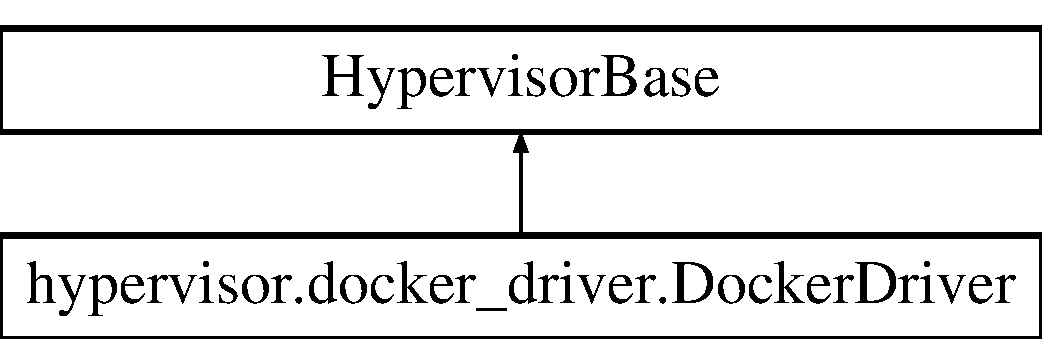
\includegraphics[height=2.000000cm]{classhypervisor_1_1docker__driver_1_1DockerDriver}
\end{center}
\end{figure}
\subsection*{Public Member Functions}
\begin{DoxyCompactItemize}
\item 
\hypertarget{classhypervisor_1_1docker__driver_1_1DockerDriver_a0b9311d90850a8a145c2961654867f98}{def {\bfseries \-\_\-\-\_\-init\-\_\-\-\_\-}}\label{classhypervisor_1_1docker__driver_1_1DockerDriver_a0b9311d90850a8a145c2961654867f98}

\item 
def \hyperlink{classhypervisor_1_1docker__driver_1_1DockerDriver_aedbd13cb76524d01894fcae539444f1b}{get\-\_\-id}
\begin{DoxyCompactList}\small\item\em Returns a container's I\-D. \end{DoxyCompactList}\item 
def \hyperlink{classhypervisor_1_1docker__driver_1_1DockerDriver_a56041a2a0afad5971b1fb5cb465b6ff6}{get\-\_\-ip}
\begin{DoxyCompactList}\small\item\em Returns a container's I\-P address. \end{DoxyCompactList}\item 
def \hyperlink{classhypervisor_1_1docker__driver_1_1DockerDriver_a9b0a6af05425f986bdc54495e9bd62c5}{deploy}
\begin{DoxyCompactList}\small\item\em Deploys a docker container. \end{DoxyCompactList}\item 
def \hyperlink{classhypervisor_1_1docker__driver_1_1DockerDriver_afe2784b21c6ef7dbe01b1188a31e9444}{start}
\begin{DoxyCompactList}\small\item\em Starts a docker container. \end{DoxyCompactList}\item 
def \hyperlink{classhypervisor_1_1docker__driver_1_1DockerDriver_abbb36db4303f0613d9013f3c2b9bfe84}{restart}
\begin{DoxyCompactList}\small\item\em Restarts a docker container. \end{DoxyCompactList}\item 
def \hyperlink{classhypervisor_1_1docker__driver_1_1DockerDriver_ab88257e3bc4660c62cd070f8de62e5a6}{stop}
\begin{DoxyCompactList}\small\item\em Stops a docker container. \end{DoxyCompactList}\item 
def \hyperlink{classhypervisor_1_1docker__driver_1_1DockerDriver_a9ffd3b0cb02e1f292a609e1d500e683f}{pause}
\begin{DoxyCompactList}\small\item\em Pauses a docker container. \end{DoxyCompactList}\item 
def \hyperlink{classhypervisor_1_1docker__driver_1_1DockerDriver_a70f14b7780fadfd2944f1518d43a9029}{unpause}
\begin{DoxyCompactList}\small\item\em Unpauses a docker container. \end{DoxyCompactList}\item 
def \hyperlink{classhypervisor_1_1docker__driver_1_1DockerDriver_ad66fd3d60fbee2760aa6b66d996eff3c}{destroy}
\begin{DoxyCompactList}\small\item\em Destroys a docker container. \end{DoxyCompactList}\item 
def \hyperlink{classhypervisor_1_1docker__driver_1_1DockerDriver_a3df8e1aeea3e30e2fef5a5d41de08159}{execute\-\_\-in\-\_\-guest}
\begin{DoxyCompactList}\small\item\em Executed commands inside a docker container. \end{DoxyCompactList}\item 
def \hyperlink{classhypervisor_1_1docker__driver_1_1DockerDriver_aabbac18594c9b6a4ee869846996c26ae}{guest\-\_\-status}
\begin{DoxyCompactList}\small\item\em Returns the status of a docker container. \end{DoxyCompactList}\end{DoxyCompactItemize}


\subsection{Detailed Description}
docker driver for nfio. 

This class provides methods for managing docker containers. 

\subsection{Member Function Documentation}
\hypertarget{classhypervisor_1_1docker__driver_1_1DockerDriver_a9b0a6af05425f986bdc54495e9bd62c5}{\index{hypervisor\-::docker\-\_\-driver\-::\-Docker\-Driver@{hypervisor\-::docker\-\_\-driver\-::\-Docker\-Driver}!deploy@{deploy}}
\index{deploy@{deploy}!hypervisor::docker_driver::DockerDriver@{hypervisor\-::docker\-\_\-driver\-::\-Docker\-Driver}}
\subsubsection[{deploy}]{\setlength{\rightskip}{0pt plus 5cm}def hypervisor.\-docker\-\_\-driver.\-Docker\-Driver.\-deploy (
\begin{DoxyParamCaption}
\item[{}]{self, }
\item[{}]{host, }
\item[{}]{user, }
\item[{}]{image\-\_\-name, }
\item[{}]{vnf\-\_\-name, }
\item[{}]{is\-\_\-privileged = {\ttfamily True}}
\end{DoxyParamCaption}
)}}\label{classhypervisor_1_1docker__driver_1_1DockerDriver_a9b0a6af05425f986bdc54495e9bd62c5}


Deploys a docker container. 


\begin{DoxyParams}{Parameters}
{\em host} & I\-P address or hostname of the machine where the docker container is to be deployed \\
\hline
{\em user} & name of the user who owns the V\-N\-F \\
\hline
{\em image\-\_\-name} & docker image name for the V\-N\-F \\
\hline
{\em vnf\-\_\-name} & name of the V\-N\-F instance \\
\hline
{\em is\-\_\-privileged} & if True then the container is deployed in privileged mode\\
\hline
\end{DoxyParams}
\begin{DoxyReturn}{Returns}
docker container I\-D 
\end{DoxyReturn}
\hypertarget{classhypervisor_1_1docker__driver_1_1DockerDriver_ad66fd3d60fbee2760aa6b66d996eff3c}{\index{hypervisor\-::docker\-\_\-driver\-::\-Docker\-Driver@{hypervisor\-::docker\-\_\-driver\-::\-Docker\-Driver}!destroy@{destroy}}
\index{destroy@{destroy}!hypervisor::docker_driver::DockerDriver@{hypervisor\-::docker\-\_\-driver\-::\-Docker\-Driver}}
\subsubsection[{destroy}]{\setlength{\rightskip}{0pt plus 5cm}def hypervisor.\-docker\-\_\-driver.\-Docker\-Driver.\-destroy (
\begin{DoxyParamCaption}
\item[{}]{self, }
\item[{}]{host, }
\item[{}]{user, }
\item[{}]{vnf\-\_\-name, }
\item[{}]{force = {\ttfamily True}}
\end{DoxyParamCaption}
)}}\label{classhypervisor_1_1docker__driver_1_1DockerDriver_ad66fd3d60fbee2760aa6b66d996eff3c}


Destroys a docker container. 


\begin{DoxyParams}{Parameters}
{\em host} & I\-P address or hostname of the machine/\-V\-M where the docker container is deployed \\
\hline
{\em user} & name of the user \\
\hline
{\em vnf\-\_\-name} & name of the V\-N\-F \\
\hline
{\em force} & if set to False then a running V\-N\-F will not be destroyed. default is True \\
\hline
\end{DoxyParams}
\hypertarget{classhypervisor_1_1docker__driver_1_1DockerDriver_a3df8e1aeea3e30e2fef5a5d41de08159}{\index{hypervisor\-::docker\-\_\-driver\-::\-Docker\-Driver@{hypervisor\-::docker\-\_\-driver\-::\-Docker\-Driver}!execute\-\_\-in\-\_\-guest@{execute\-\_\-in\-\_\-guest}}
\index{execute\-\_\-in\-\_\-guest@{execute\-\_\-in\-\_\-guest}!hypervisor::docker_driver::DockerDriver@{hypervisor\-::docker\-\_\-driver\-::\-Docker\-Driver}}
\subsubsection[{execute\-\_\-in\-\_\-guest}]{\setlength{\rightskip}{0pt plus 5cm}def hypervisor.\-docker\-\_\-driver.\-Docker\-Driver.\-execute\-\_\-in\-\_\-guest (
\begin{DoxyParamCaption}
\item[{}]{self, }
\item[{}]{host, }
\item[{}]{user, }
\item[{}]{vnf\-\_\-name, }
\item[{}]{cmd}
\end{DoxyParamCaption}
)}}\label{classhypervisor_1_1docker__driver_1_1DockerDriver_a3df8e1aeea3e30e2fef5a5d41de08159}


Executed commands inside a docker container. 


\begin{DoxyParams}{Parameters}
{\em host} & I\-P address or hostname of the machine/\-V\-M where the docker container is deployed \\
\hline
{\em user} & name of the user \\
\hline
{\em vnf\-\_\-name} & name of the V\-N\-F \\
\hline
{\em cmd} & the command to execute inside the container\\
\hline
\end{DoxyParams}
\begin{DoxyReturn}{Returns}
The output of the command passes as cmd 
\end{DoxyReturn}
\hypertarget{classhypervisor_1_1docker__driver_1_1DockerDriver_aedbd13cb76524d01894fcae539444f1b}{\index{hypervisor\-::docker\-\_\-driver\-::\-Docker\-Driver@{hypervisor\-::docker\-\_\-driver\-::\-Docker\-Driver}!get\-\_\-id@{get\-\_\-id}}
\index{get\-\_\-id@{get\-\_\-id}!hypervisor::docker_driver::DockerDriver@{hypervisor\-::docker\-\_\-driver\-::\-Docker\-Driver}}
\subsubsection[{get\-\_\-id}]{\setlength{\rightskip}{0pt plus 5cm}def hypervisor.\-docker\-\_\-driver.\-Docker\-Driver.\-get\-\_\-id (
\begin{DoxyParamCaption}
\item[{}]{self, }
\item[{}]{host, }
\item[{}]{user, }
\item[{}]{vnf\-\_\-name}
\end{DoxyParamCaption}
)}}\label{classhypervisor_1_1docker__driver_1_1DockerDriver_aedbd13cb76524d01894fcae539444f1b}


Returns a container's I\-D. 


\begin{DoxyParams}{Parameters}
{\em host} & I\-P address or hostname of the machine where the docker container is deployed \\
\hline
{\em user} & name of the user who owns the V\-N\-F \\
\hline
{\em vnf\-\_\-name} & name of the V\-N\-F instance whose I\-D is being queried\\
\hline
\end{DoxyParams}
\begin{DoxyReturn}{Returns}
docker container I\-D. 
\end{DoxyReturn}
\hypertarget{classhypervisor_1_1docker__driver_1_1DockerDriver_a56041a2a0afad5971b1fb5cb465b6ff6}{\index{hypervisor\-::docker\-\_\-driver\-::\-Docker\-Driver@{hypervisor\-::docker\-\_\-driver\-::\-Docker\-Driver}!get\-\_\-ip@{get\-\_\-ip}}
\index{get\-\_\-ip@{get\-\_\-ip}!hypervisor::docker_driver::DockerDriver@{hypervisor\-::docker\-\_\-driver\-::\-Docker\-Driver}}
\subsubsection[{get\-\_\-ip}]{\setlength{\rightskip}{0pt plus 5cm}def hypervisor.\-docker\-\_\-driver.\-Docker\-Driver.\-get\-\_\-ip (
\begin{DoxyParamCaption}
\item[{}]{self, }
\item[{}]{host, }
\item[{}]{user, }
\item[{}]{vnf\-\_\-name}
\end{DoxyParamCaption}
)}}\label{classhypervisor_1_1docker__driver_1_1DockerDriver_a56041a2a0afad5971b1fb5cb465b6ff6}


Returns a container's I\-P address. 


\begin{DoxyParams}{Parameters}
{\em host} & I\-P address or hostname of the machine where the docker container is deployed \\
\hline
{\em user} & name of the user who owns the V\-N\-F \\
\hline
{\em vnf\-\_\-name} & name of the V\-N\-F instance whose I\-D is being queried\\
\hline
\end{DoxyParams}
\begin{DoxyReturn}{Returns}
docker container's I\-P. 
\end{DoxyReturn}
\hypertarget{classhypervisor_1_1docker__driver_1_1DockerDriver_aabbac18594c9b6a4ee869846996c26ae}{\index{hypervisor\-::docker\-\_\-driver\-::\-Docker\-Driver@{hypervisor\-::docker\-\_\-driver\-::\-Docker\-Driver}!guest\-\_\-status@{guest\-\_\-status}}
\index{guest\-\_\-status@{guest\-\_\-status}!hypervisor::docker_driver::DockerDriver@{hypervisor\-::docker\-\_\-driver\-::\-Docker\-Driver}}
\subsubsection[{guest\-\_\-status}]{\setlength{\rightskip}{0pt plus 5cm}def hypervisor.\-docker\-\_\-driver.\-Docker\-Driver.\-guest\-\_\-status (
\begin{DoxyParamCaption}
\item[{}]{self, }
\item[{}]{host, }
\item[{}]{user, }
\item[{}]{vnf\-\_\-name}
\end{DoxyParamCaption}
)}}\label{classhypervisor_1_1docker__driver_1_1DockerDriver_aabbac18594c9b6a4ee869846996c26ae}


Returns the status of a docker container. 


\begin{DoxyParams}{Parameters}
{\em host} & I\-P address or hostname of the machine/\-V\-M where the docker container is deployed \\
\hline
{\em user} & name of the user \\
\hline
{\em vnf\-\_\-name} & name of the V\-N\-F\\
\hline
\end{DoxyParams}
\begin{DoxyReturn}{Returns}
current state of the docker container 
\end{DoxyReturn}
\hypertarget{classhypervisor_1_1docker__driver_1_1DockerDriver_a9ffd3b0cb02e1f292a609e1d500e683f}{\index{hypervisor\-::docker\-\_\-driver\-::\-Docker\-Driver@{hypervisor\-::docker\-\_\-driver\-::\-Docker\-Driver}!pause@{pause}}
\index{pause@{pause}!hypervisor::docker_driver::DockerDriver@{hypervisor\-::docker\-\_\-driver\-::\-Docker\-Driver}}
\subsubsection[{pause}]{\setlength{\rightskip}{0pt plus 5cm}def hypervisor.\-docker\-\_\-driver.\-Docker\-Driver.\-pause (
\begin{DoxyParamCaption}
\item[{}]{self, }
\item[{}]{host, }
\item[{}]{user, }
\item[{}]{vnf\-\_\-name}
\end{DoxyParamCaption}
)}}\label{classhypervisor_1_1docker__driver_1_1DockerDriver_a9ffd3b0cb02e1f292a609e1d500e683f}


Pauses a docker container. 


\begin{DoxyParams}{Parameters}
{\em host} & I\-P address or hostname of the machine/\-V\-M where the docker container is deployed \\
\hline
{\em user} & name of the user \\
\hline
{\em vnf\-\_\-name} & name of the V\-N\-F \\
\hline
\end{DoxyParams}
\hypertarget{classhypervisor_1_1docker__driver_1_1DockerDriver_abbb36db4303f0613d9013f3c2b9bfe84}{\index{hypervisor\-::docker\-\_\-driver\-::\-Docker\-Driver@{hypervisor\-::docker\-\_\-driver\-::\-Docker\-Driver}!restart@{restart}}
\index{restart@{restart}!hypervisor::docker_driver::DockerDriver@{hypervisor\-::docker\-\_\-driver\-::\-Docker\-Driver}}
\subsubsection[{restart}]{\setlength{\rightskip}{0pt plus 5cm}def hypervisor.\-docker\-\_\-driver.\-Docker\-Driver.\-restart (
\begin{DoxyParamCaption}
\item[{}]{self, }
\item[{}]{host, }
\item[{}]{user, }
\item[{}]{vnf\-\_\-name}
\end{DoxyParamCaption}
)}}\label{classhypervisor_1_1docker__driver_1_1DockerDriver_abbb36db4303f0613d9013f3c2b9bfe84}


Restarts a docker container. 


\begin{DoxyParams}{Parameters}
{\em host} & I\-P address or hostname of the machine/\-V\-M where the docker container is deployed \\
\hline
{\em user} & name of the user \\
\hline
{\em vnf\-\_\-name} & name of the V\-N\-F \\
\hline
\end{DoxyParams}
\hypertarget{classhypervisor_1_1docker__driver_1_1DockerDriver_afe2784b21c6ef7dbe01b1188a31e9444}{\index{hypervisor\-::docker\-\_\-driver\-::\-Docker\-Driver@{hypervisor\-::docker\-\_\-driver\-::\-Docker\-Driver}!start@{start}}
\index{start@{start}!hypervisor::docker_driver::DockerDriver@{hypervisor\-::docker\-\_\-driver\-::\-Docker\-Driver}}
\subsubsection[{start}]{\setlength{\rightskip}{0pt plus 5cm}def hypervisor.\-docker\-\_\-driver.\-Docker\-Driver.\-start (
\begin{DoxyParamCaption}
\item[{}]{self, }
\item[{}]{host, }
\item[{}]{user, }
\item[{}]{vnf\-\_\-name, }
\item[{}]{is\-\_\-privileged = {\ttfamily True}}
\end{DoxyParamCaption}
)}}\label{classhypervisor_1_1docker__driver_1_1DockerDriver_afe2784b21c6ef7dbe01b1188a31e9444}


Starts a docker container. 


\begin{DoxyParams}{Parameters}
{\em host} & I\-P address or hostname of the machine/\-V\-M where the docker container is deployed \\
\hline
{\em user} & name of the user \\
\hline
{\em vnf\-\_\-name} & name of the V\-N\-F \\
\hline
{\em is\-\_\-privileged} & if True then the container is started in privileged mode \\
\hline
\end{DoxyParams}
\hypertarget{classhypervisor_1_1docker__driver_1_1DockerDriver_ab88257e3bc4660c62cd070f8de62e5a6}{\index{hypervisor\-::docker\-\_\-driver\-::\-Docker\-Driver@{hypervisor\-::docker\-\_\-driver\-::\-Docker\-Driver}!stop@{stop}}
\index{stop@{stop}!hypervisor::docker_driver::DockerDriver@{hypervisor\-::docker\-\_\-driver\-::\-Docker\-Driver}}
\subsubsection[{stop}]{\setlength{\rightskip}{0pt plus 5cm}def hypervisor.\-docker\-\_\-driver.\-Docker\-Driver.\-stop (
\begin{DoxyParamCaption}
\item[{}]{self, }
\item[{}]{host, }
\item[{}]{user, }
\item[{}]{vnf\-\_\-name}
\end{DoxyParamCaption}
)}}\label{classhypervisor_1_1docker__driver_1_1DockerDriver_ab88257e3bc4660c62cd070f8de62e5a6}


Stops a docker container. 


\begin{DoxyParams}{Parameters}
{\em host} & I\-P address or hostname of the machine/\-V\-M where the docker container is deployed \\
\hline
{\em user} & name of the user \\
\hline
{\em vnf\-\_\-name} & name of the V\-N\-F \\
\hline
\end{DoxyParams}
\hypertarget{classhypervisor_1_1docker__driver_1_1DockerDriver_a70f14b7780fadfd2944f1518d43a9029}{\index{hypervisor\-::docker\-\_\-driver\-::\-Docker\-Driver@{hypervisor\-::docker\-\_\-driver\-::\-Docker\-Driver}!unpause@{unpause}}
\index{unpause@{unpause}!hypervisor::docker_driver::DockerDriver@{hypervisor\-::docker\-\_\-driver\-::\-Docker\-Driver}}
\subsubsection[{unpause}]{\setlength{\rightskip}{0pt plus 5cm}def hypervisor.\-docker\-\_\-driver.\-Docker\-Driver.\-unpause (
\begin{DoxyParamCaption}
\item[{}]{self, }
\item[{}]{host, }
\item[{}]{user, }
\item[{}]{vnf\-\_\-name}
\end{DoxyParamCaption}
)}}\label{classhypervisor_1_1docker__driver_1_1DockerDriver_a70f14b7780fadfd2944f1518d43a9029}


Unpauses a docker container. 


\begin{DoxyParams}{Parameters}
{\em host} & I\-P address or hostname of the machine/\-V\-M where the docker container is deployed \\
\hline
{\em user} & name of the user \\
\hline
{\em vnf\-\_\-name} & name of the V\-N\-F \\
\hline
\end{DoxyParams}


The documentation for this class was generated from the following file\-:\begin{DoxyCompactItemize}
\item 
Wat\-N\-F\-V/nf.\-io/src/hypervisor/docker\-\_\-driver.\-py\end{DoxyCompactItemize}

\hypertarget{classhypervisor_1_1hypervisor__base_1_1HypervisorBase}{\section{hypervisor.\-hypervisor\-\_\-base.\-Hypervisor\-Base Class Reference}
\label{classhypervisor_1_1hypervisor__base_1_1HypervisorBase}\index{hypervisor.\-hypervisor\-\_\-base.\-Hypervisor\-Base@{hypervisor.\-hypervisor\-\_\-base.\-Hypervisor\-Base}}
}


Base class for hypervisors.  


Inheritance diagram for hypervisor.\-hypervisor\-\_\-base.\-Hypervisor\-Base\-:\begin{figure}[H]
\begin{center}
\leavevmode
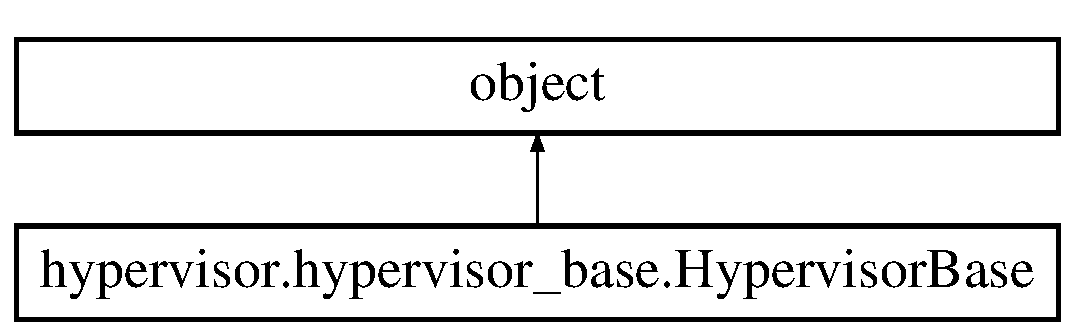
\includegraphics[height=2.000000cm]{classhypervisor_1_1hypervisor__base_1_1HypervisorBase}
\end{center}
\end{figure}
\subsection*{Public Member Functions}
\begin{DoxyCompactItemize}
\item 
def \hyperlink{classhypervisor_1_1hypervisor__base_1_1HypervisorBase_aa06a6d5c765f477edc9b2121aa1477f8}{get\-\_\-id}
\begin{DoxyCompactList}\small\item\em Returns the hypervisor specific I\-D of the V\-M or container. \end{DoxyCompactList}\item 
def \hyperlink{classhypervisor_1_1hypervisor__base_1_1HypervisorBase_aaaecc9f6059daebb99596f7bae3b4c61}{deploy}
\begin{DoxyCompactList}\small\item\em Deploys a V\-M or continer. \end{DoxyCompactList}\item 
def \hyperlink{classhypervisor_1_1hypervisor__base_1_1HypervisorBase_ab4147962f621e47480a67da9dbab6ec7}{pause}
\begin{DoxyCompactList}\small\item\em Pauses a V\-M or continer. \end{DoxyCompactList}\item 
def \hyperlink{classhypervisor_1_1hypervisor__base_1_1HypervisorBase_a9fb778f97170ab9b0248a5048261f53e}{destroy}
\begin{DoxyCompactList}\small\item\em Destroys a V\-M or continer. \end{DoxyCompactList}\item 
def \hyperlink{classhypervisor_1_1hypervisor__base_1_1HypervisorBase_ab73d82fec1cbeadcc3b859310ebcf16e}{execute\-\_\-in\-\_\-guest}
\begin{DoxyCompactList}\small\item\em Executes a command in the V\-M or continer. \end{DoxyCompactList}\item 
def \hyperlink{classhypervisor_1_1hypervisor__base_1_1HypervisorBase_a4891d99be2c92c1082eab91b82a4ddad}{guest\-\_\-status}
\begin{DoxyCompactList}\small\item\em Returns the current status of a V\-M or continer. \end{DoxyCompactList}\end{DoxyCompactItemize}


\subsection{Detailed Description}
Base class for hypervisors. 

This class must be extended by a hypervisor driver. 

\subsection{Member Function Documentation}
\hypertarget{classhypervisor_1_1hypervisor__base_1_1HypervisorBase_aaaecc9f6059daebb99596f7bae3b4c61}{\index{hypervisor\-::hypervisor\-\_\-base\-::\-Hypervisor\-Base@{hypervisor\-::hypervisor\-\_\-base\-::\-Hypervisor\-Base}!deploy@{deploy}}
\index{deploy@{deploy}!hypervisor::hypervisor_base::HypervisorBase@{hypervisor\-::hypervisor\-\_\-base\-::\-Hypervisor\-Base}}
\subsubsection[{deploy}]{\setlength{\rightskip}{0pt plus 5cm}def hypervisor.\-hypervisor\-\_\-base.\-Hypervisor\-Base.\-deploy (
\begin{DoxyParamCaption}
\item[{}]{self}
\end{DoxyParamCaption}
)}}\label{classhypervisor_1_1hypervisor__base_1_1HypervisorBase_aaaecc9f6059daebb99596f7bae3b4c61}


Deploys a V\-M or continer. 

Args\-: Defined in derived class.

Returns\-: Hypervisor specific return code. \hypertarget{classhypervisor_1_1hypervisor__base_1_1HypervisorBase_a9fb778f97170ab9b0248a5048261f53e}{\index{hypervisor\-::hypervisor\-\_\-base\-::\-Hypervisor\-Base@{hypervisor\-::hypervisor\-\_\-base\-::\-Hypervisor\-Base}!destroy@{destroy}}
\index{destroy@{destroy}!hypervisor::hypervisor_base::HypervisorBase@{hypervisor\-::hypervisor\-\_\-base\-::\-Hypervisor\-Base}}
\subsubsection[{destroy}]{\setlength{\rightskip}{0pt plus 5cm}def hypervisor.\-hypervisor\-\_\-base.\-Hypervisor\-Base.\-destroy (
\begin{DoxyParamCaption}
\item[{}]{self}
\end{DoxyParamCaption}
)}}\label{classhypervisor_1_1hypervisor__base_1_1HypervisorBase_a9fb778f97170ab9b0248a5048261f53e}


Destroys a V\-M or continer. 

Args\-: Defined in derived class.

Returns\-: Hypervisor specific return code. \hypertarget{classhypervisor_1_1hypervisor__base_1_1HypervisorBase_ab73d82fec1cbeadcc3b859310ebcf16e}{\index{hypervisor\-::hypervisor\-\_\-base\-::\-Hypervisor\-Base@{hypervisor\-::hypervisor\-\_\-base\-::\-Hypervisor\-Base}!execute\-\_\-in\-\_\-guest@{execute\-\_\-in\-\_\-guest}}
\index{execute\-\_\-in\-\_\-guest@{execute\-\_\-in\-\_\-guest}!hypervisor::hypervisor_base::HypervisorBase@{hypervisor\-::hypervisor\-\_\-base\-::\-Hypervisor\-Base}}
\subsubsection[{execute\-\_\-in\-\_\-guest}]{\setlength{\rightskip}{0pt plus 5cm}def hypervisor.\-hypervisor\-\_\-base.\-Hypervisor\-Base.\-execute\-\_\-in\-\_\-guest (
\begin{DoxyParamCaption}
\item[{}]{self}
\end{DoxyParamCaption}
)}}\label{classhypervisor_1_1hypervisor__base_1_1HypervisorBase_ab73d82fec1cbeadcc3b859310ebcf16e}


Executes a command in the V\-M or continer. 

Args\-: Defined in derived class.

Returns\-: Hypervisor specific return code. \hypertarget{classhypervisor_1_1hypervisor__base_1_1HypervisorBase_aa06a6d5c765f477edc9b2121aa1477f8}{\index{hypervisor\-::hypervisor\-\_\-base\-::\-Hypervisor\-Base@{hypervisor\-::hypervisor\-\_\-base\-::\-Hypervisor\-Base}!get\-\_\-id@{get\-\_\-id}}
\index{get\-\_\-id@{get\-\_\-id}!hypervisor::hypervisor_base::HypervisorBase@{hypervisor\-::hypervisor\-\_\-base\-::\-Hypervisor\-Base}}
\subsubsection[{get\-\_\-id}]{\setlength{\rightskip}{0pt plus 5cm}def hypervisor.\-hypervisor\-\_\-base.\-Hypervisor\-Base.\-get\-\_\-id (
\begin{DoxyParamCaption}
\item[{}]{self}
\end{DoxyParamCaption}
)}}\label{classhypervisor_1_1hypervisor__base_1_1HypervisorBase_aa06a6d5c765f477edc9b2121aa1477f8}


Returns the hypervisor specific I\-D of the V\-M or container. 

Args\-: Defined in derived class.

Returns\-: Hypervisor specific I\-D for a V\-M or container. \hypertarget{classhypervisor_1_1hypervisor__base_1_1HypervisorBase_a4891d99be2c92c1082eab91b82a4ddad}{\index{hypervisor\-::hypervisor\-\_\-base\-::\-Hypervisor\-Base@{hypervisor\-::hypervisor\-\_\-base\-::\-Hypervisor\-Base}!guest\-\_\-status@{guest\-\_\-status}}
\index{guest\-\_\-status@{guest\-\_\-status}!hypervisor::hypervisor_base::HypervisorBase@{hypervisor\-::hypervisor\-\_\-base\-::\-Hypervisor\-Base}}
\subsubsection[{guest\-\_\-status}]{\setlength{\rightskip}{0pt plus 5cm}def hypervisor.\-hypervisor\-\_\-base.\-Hypervisor\-Base.\-guest\-\_\-status (
\begin{DoxyParamCaption}
\item[{}]{self}
\end{DoxyParamCaption}
)}}\label{classhypervisor_1_1hypervisor__base_1_1HypervisorBase_a4891d99be2c92c1082eab91b82a4ddad}


Returns the current status of a V\-M or continer. 

Args\-: Defined in derived class.

Returns\-: Current status of a V\-M or container. \hypertarget{classhypervisor_1_1hypervisor__base_1_1HypervisorBase_ab4147962f621e47480a67da9dbab6ec7}{\index{hypervisor\-::hypervisor\-\_\-base\-::\-Hypervisor\-Base@{hypervisor\-::hypervisor\-\_\-base\-::\-Hypervisor\-Base}!pause@{pause}}
\index{pause@{pause}!hypervisor::hypervisor_base::HypervisorBase@{hypervisor\-::hypervisor\-\_\-base\-::\-Hypervisor\-Base}}
\subsubsection[{pause}]{\setlength{\rightskip}{0pt plus 5cm}def hypervisor.\-hypervisor\-\_\-base.\-Hypervisor\-Base.\-pause (
\begin{DoxyParamCaption}
\item[{}]{self}
\end{DoxyParamCaption}
)}}\label{classhypervisor_1_1hypervisor__base_1_1HypervisorBase_ab4147962f621e47480a67da9dbab6ec7}


Pauses a V\-M or continer. 

Args\-: Defined in derived class.

Returns\-: Hypervisor specific return code. 

The documentation for this class was generated from the following file\-:\begin{DoxyCompactItemize}
\item 
/home/nfuser/nf.\-io/src/hypervisor/hypervisor\-\_\-base.\-py\end{DoxyCompactItemize}

\hypertarget{classerrors_1_1HypervisorConnectionError}{\section{errors.\-Hypervisor\-Connection\-Error Class Reference}
\label{classerrors_1_1HypervisorConnectionError}\index{errors.\-Hypervisor\-Connection\-Error@{errors.\-Hypervisor\-Connection\-Error}}
}
Inheritance diagram for errors.\-Hypervisor\-Connection\-Error\-:\begin{figure}[H]
\begin{center}
\leavevmode
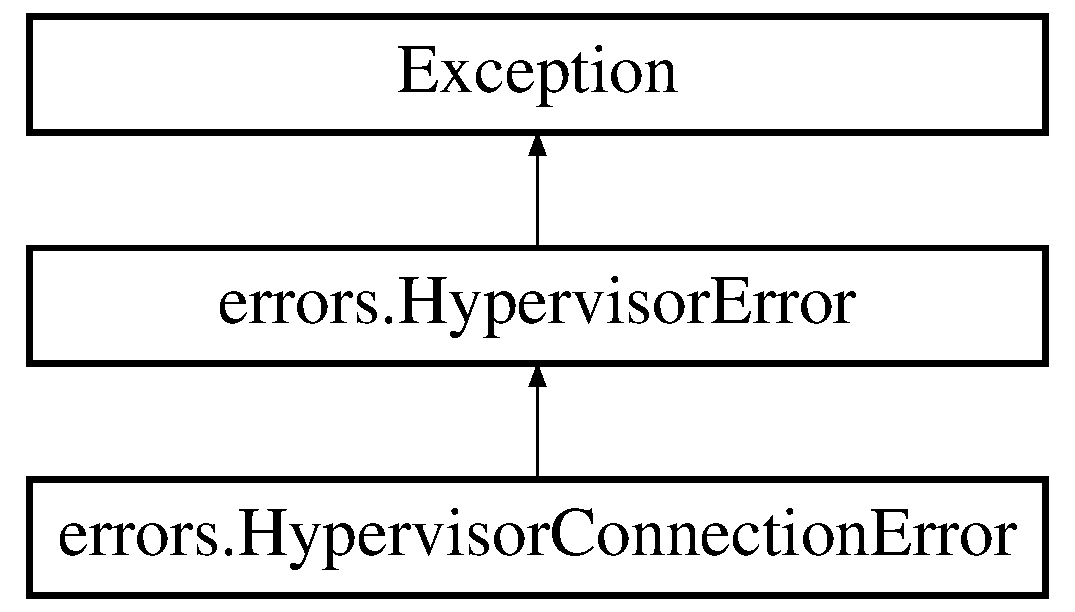
\includegraphics[height=4.000000cm]{classerrors_1_1HypervisorConnectionError}
\end{center}
\end{figure}
\subsection*{Public Member Functions}
\begin{DoxyCompactItemize}
\item 
\hypertarget{classerrors_1_1HypervisorConnectionError_a8ac18f912e2fa2866649688a43acc42c}{def {\bfseries \-\_\-\-\_\-init\-\_\-\-\_\-}}\label{classerrors_1_1HypervisorConnectionError_a8ac18f912e2fa2866649688a43acc42c}

\end{DoxyCompactItemize}
\subsection*{Public Attributes}
\begin{DoxyCompactItemize}
\item 
\hypertarget{classerrors_1_1HypervisorConnectionError_a4f3ea14dba51da58bf328573f69eabb4}{{\bfseries errno}}\label{classerrors_1_1HypervisorConnectionError_a4f3ea14dba51da58bf328573f69eabb4}

\end{DoxyCompactItemize}


\subsection{Detailed Description}


Definition at line 15 of file errors.\-py.



The documentation for this class was generated from the following file\-:\begin{DoxyCompactItemize}
\item 
Wat\-N\-F\-V/nf.\-io/src/errors.\-py\end{DoxyCompactItemize}

\hypertarget{classerrors_1_1HypervisorError}{\section{errors.\-Hypervisor\-Error Class Reference}
\label{classerrors_1_1HypervisorError}\index{errors.\-Hypervisor\-Error@{errors.\-Hypervisor\-Error}}
}
Inheritance diagram for errors.\-Hypervisor\-Error\-:\begin{figure}[H]
\begin{center}
\leavevmode
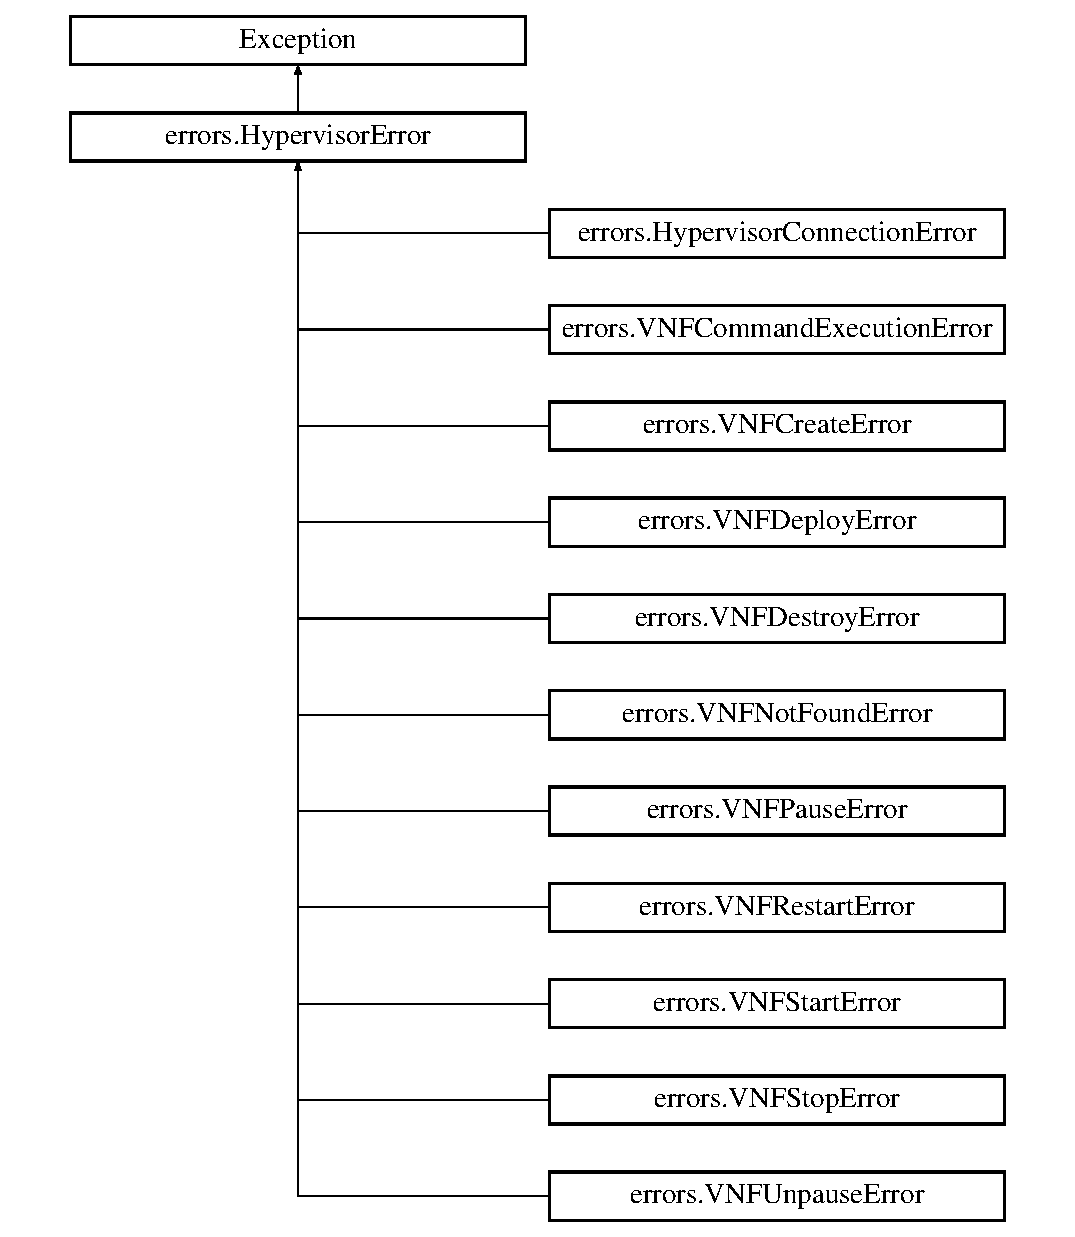
\includegraphics[height=12.000000cm]{classerrors_1_1HypervisorError}
\end{center}
\end{figure}


\subsection{Detailed Description}


Definition at line 9 of file errors.\-py.



The documentation for this class was generated from the following file\-:\begin{DoxyCompactItemize}
\item 
Wat\-N\-F\-V/nf.\-io/src/errors.\-py\end{DoxyCompactItemize}

\hypertarget{classhypervisor_1_1hypervisor__factory_1_1HypervisorFactory}{\section{hypervisor.\-hypervisor\-\_\-factory.\-Hypervisor\-Factory Class Reference}
\label{classhypervisor_1_1hypervisor__factory_1_1HypervisorFactory}\index{hypervisor.\-hypervisor\-\_\-factory.\-Hypervisor\-Factory@{hypervisor.\-hypervisor\-\_\-factory.\-Hypervisor\-Factory}}
}
Inheritance diagram for hypervisor.\-hypervisor\-\_\-factory.\-Hypervisor\-Factory\-:\begin{figure}[H]
\begin{center}
\leavevmode
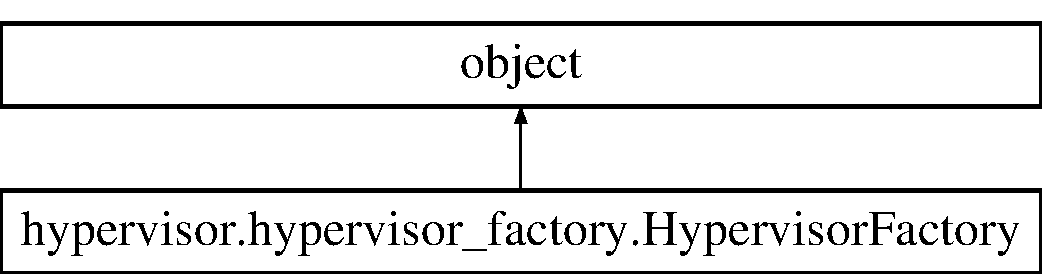
\includegraphics[height=2.000000cm]{classhypervisor_1_1hypervisor__factory_1_1HypervisorFactory}
\end{center}
\end{figure}
\subsection*{Public Member Functions}
\begin{DoxyCompactItemize}
\item 
\hypertarget{classhypervisor_1_1hypervisor__factory_1_1HypervisorFactory_ab1691cc3620d76c0a266e0fd469548ad}{def {\bfseries \-\_\-\-\_\-init\-\_\-\-\_\-}}\label{classhypervisor_1_1hypervisor__factory_1_1HypervisorFactory_ab1691cc3620d76c0a266e0fd469548ad}

\end{DoxyCompactItemize}
\subsection*{Static Public Member Functions}
\begin{DoxyCompactItemize}
\item 
\hypertarget{classhypervisor_1_1hypervisor__factory_1_1HypervisorFactory_ade4356e4251e644d580f8c1c53fc704e}{def {\bfseries get\-\_\-hypervisor\-\_\-instance}}\label{classhypervisor_1_1hypervisor__factory_1_1HypervisorFactory_ade4356e4251e644d580f8c1c53fc704e}

\end{DoxyCompactItemize}


The documentation for this class was generated from the following file\-:\begin{DoxyCompactItemize}
\item 
/home/mfbari/works/\-Wat\-N\-F\-V/nf.\-io/src/hypervisor/hypervisor\-\_\-factory.\-py\end{DoxyCompactItemize}

\hypertarget{classhypervisor_1_1libvirt__driver_1_1Libvirt}{\section{hypervisor.\-libvirt\-\_\-driver.\-Libvirt Class Reference}
\label{classhypervisor_1_1libvirt__driver_1_1Libvirt}\index{hypervisor.\-libvirt\-\_\-driver.\-Libvirt@{hypervisor.\-libvirt\-\_\-driver.\-Libvirt}}
}
Inheritance diagram for hypervisor.\-libvirt\-\_\-driver.\-Libvirt\-:\begin{figure}[H]
\begin{center}
\leavevmode
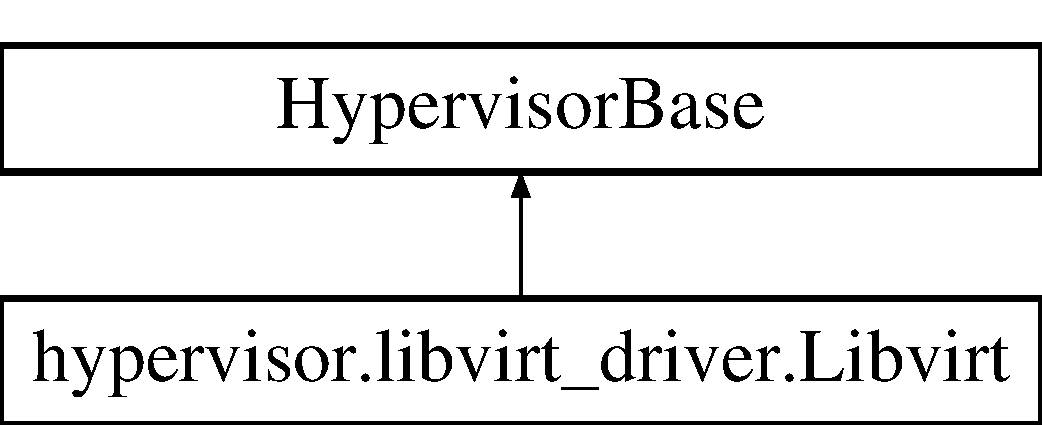
\includegraphics[height=2.000000cm]{classhypervisor_1_1libvirt__driver_1_1Libvirt}
\end{center}
\end{figure}
\subsection*{Public Member Functions}
\begin{DoxyCompactItemize}
\item 
\hypertarget{classhypervisor_1_1libvirt__driver_1_1Libvirt_ab8f6a87c28e570ecc55693e665b915fa}{def {\bfseries deploy}}\label{classhypervisor_1_1libvirt__driver_1_1Libvirt_ab8f6a87c28e570ecc55693e665b915fa}

\item 
\hypertarget{classhypervisor_1_1libvirt__driver_1_1Libvirt_ae82b6fcef27839a8db06edfb0857ee9e}{def {\bfseries pause}}\label{classhypervisor_1_1libvirt__driver_1_1Libvirt_ae82b6fcef27839a8db06edfb0857ee9e}

\item 
\hypertarget{classhypervisor_1_1libvirt__driver_1_1Libvirt_a48a5b9aa63f54fff5c4bcfd2dbdf104a}{def {\bfseries destroy}}\label{classhypervisor_1_1libvirt__driver_1_1Libvirt_a48a5b9aa63f54fff5c4bcfd2dbdf104a}

\end{DoxyCompactItemize}


The documentation for this class was generated from the following file\-:\begin{DoxyCompactItemize}
\item 
Wat\-N\-F\-V/nf.\-io/src/hypervisor/libvirt\-\_\-driver.\-py\end{DoxyCompactItemize}

\hypertarget{classnfio_1_1Nfio}{\section{nfio.\-Nfio Class Reference}
\label{classnfio_1_1Nfio}\index{nfio.\-Nfio@{nfio.\-Nfio}}
}
Inheritance diagram for nfio.\-Nfio\-:\begin{figure}[H]
\begin{center}
\leavevmode
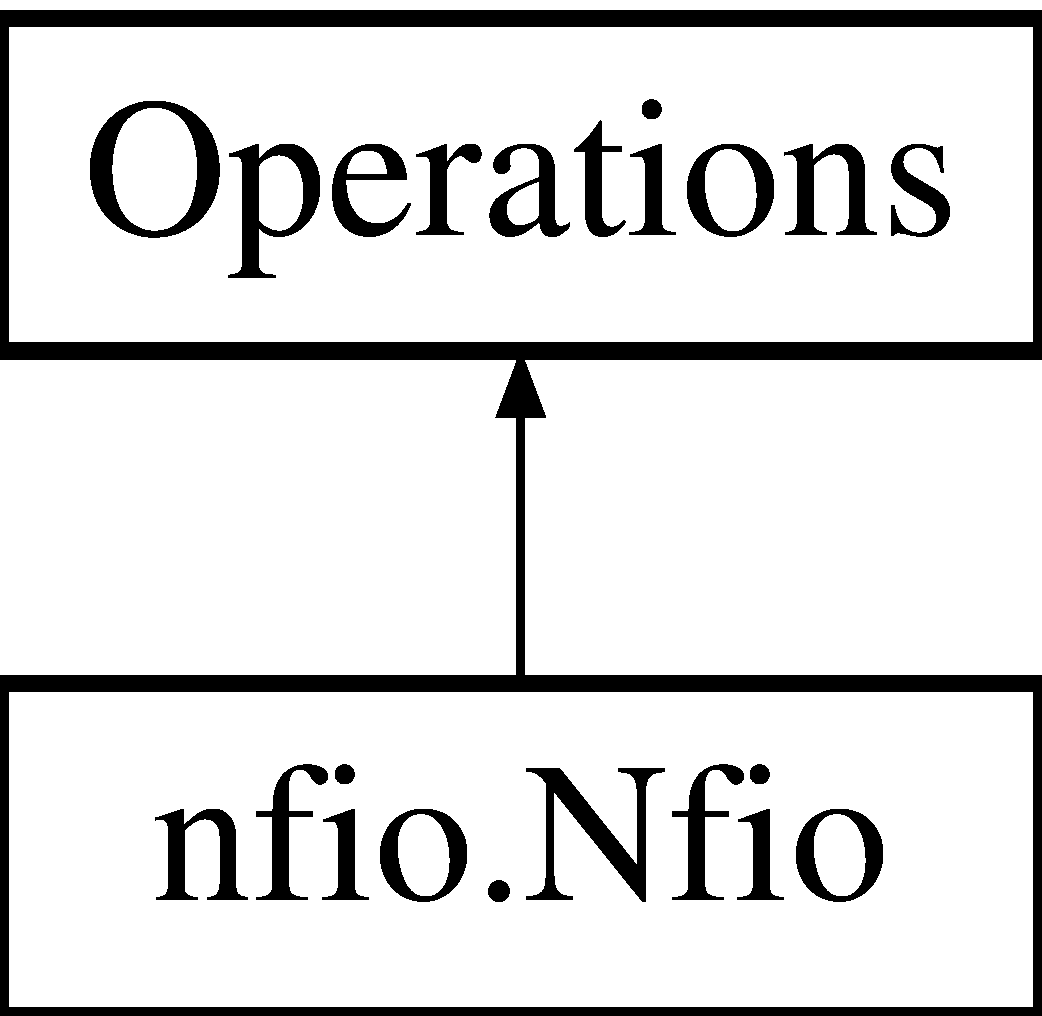
\includegraphics[height=3.000000cm]{classnfio_1_1Nfio}
\end{center}
\end{figure}
\subsection*{Public Member Functions}
\begin{DoxyCompactItemize}
\item 
def \hyperlink{classnfio_1_1Nfio_a37d06beb4658927077f41fdfd237c2b1}{\-\_\-\-\_\-init\-\_\-\-\_\-}
\begin{DoxyCompactList}\small\item\em Instantiates a \hyperlink{classnfio_1_1Nfio}{Nfio} object. \end{DoxyCompactList}\item 
\hypertarget{classnfio_1_1Nfio_a73f04474e4c327027cc36e9a27d8d37d}{def {\bfseries access}}\label{classnfio_1_1Nfio_a73f04474e4c327027cc36e9a27d8d37d}

\item 
\hypertarget{classnfio_1_1Nfio_a0e1a2a60c6ad3552b9e737bf5c21b298}{def {\bfseries chmod}}\label{classnfio_1_1Nfio_a0e1a2a60c6ad3552b9e737bf5c21b298}

\item 
\hypertarget{classnfio_1_1Nfio_a69cc0d977007fc2057f167acfd484293}{def {\bfseries chown}}\label{classnfio_1_1Nfio_a69cc0d977007fc2057f167acfd484293}

\item 
def \hyperlink{classnfio_1_1Nfio_a46d186e9d92c1fea58a01ffc08ebb5dc}{getattr}
\begin{DoxyCompactList}\small\item\em Returns the file attributes of the file specified by path Args\-: path\-: Path of the file fh\-: Open file handle to the file Returns\-: A dictionary containing file attributes. \end{DoxyCompactList}\item 
\hypertarget{classnfio_1_1Nfio_a648947134659a41ad9b2b68d1aa7edfe}{def {\bfseries readdir}}\label{classnfio_1_1Nfio_a648947134659a41ad9b2b68d1aa7edfe}

\item 
\hypertarget{classnfio_1_1Nfio_a28f5eba4c82e6b5d7fb13654eb97cb8f}{def {\bfseries readlink}}\label{classnfio_1_1Nfio_a28f5eba4c82e6b5d7fb13654eb97cb8f}

\item 
\hypertarget{classnfio_1_1Nfio_ab34cbc64205b1932d86b6f79063710e4}{def {\bfseries mknod}}\label{classnfio_1_1Nfio_ab34cbc64205b1932d86b6f79063710e4}

\item 
\hypertarget{classnfio_1_1Nfio_afb377c76425223681e5aa703d75fc6ac}{def {\bfseries rmdir}}\label{classnfio_1_1Nfio_afb377c76425223681e5aa703d75fc6ac}

\item 
def \hyperlink{classnfio_1_1Nfio_a03f752db91f0335cf0f29d81bda84b66}{mkdir}
\begin{DoxyCompactList}\small\item\em The semantics have been redefined to create a new V\-N\-F instance when a directory is created under a specific type of V\-N\-F directory. \end{DoxyCompactList}\item 
\hypertarget{classnfio_1_1Nfio_a65835e246a89861440548951f75278a8}{def {\bfseries statfs}}\label{classnfio_1_1Nfio_a65835e246a89861440548951f75278a8}

\item 
\hypertarget{classnfio_1_1Nfio_a316c7dd77e736d1db3c4f1d4ce752b5e}{def {\bfseries unlink}}\label{classnfio_1_1Nfio_a316c7dd77e736d1db3c4f1d4ce752b5e}

\item 
\hypertarget{classnfio_1_1Nfio_a67a77270fc5247a10d9e170f7f554139}{def {\bfseries symlink}}\label{classnfio_1_1Nfio_a67a77270fc5247a10d9e170f7f554139}

\item 
\hypertarget{classnfio_1_1Nfio_aec88d98d0a363cda41f0df74fab80d23}{def {\bfseries rename}}\label{classnfio_1_1Nfio_aec88d98d0a363cda41f0df74fab80d23}

\item 
\hypertarget{classnfio_1_1Nfio_ad56e16263c502849dcb2a32d8d8d42de}{def {\bfseries link}}\label{classnfio_1_1Nfio_ad56e16263c502849dcb2a32d8d8d42de}

\item 
\hypertarget{classnfio_1_1Nfio_a4614e16989b90bd79c6610211ae1694b}{def {\bfseries utimens}}\label{classnfio_1_1Nfio_a4614e16989b90bd79c6610211ae1694b}

\item 
\hypertarget{classnfio_1_1Nfio_a7f8141a10d199e0c7d4da91727fb2767}{def {\bfseries open}}\label{classnfio_1_1Nfio_a7f8141a10d199e0c7d4da91727fb2767}

\item 
\hypertarget{classnfio_1_1Nfio_a157f53007ef2e2afb63ee80e84f52eff}{def {\bfseries create}}\label{classnfio_1_1Nfio_a157f53007ef2e2afb63ee80e84f52eff}

\item 
def \hyperlink{classnfio_1_1Nfio_aa96de630c8da283fe30851e8d7b378a3}{read}
\begin{DoxyCompactList}\small\item\em Reads an open file. \end{DoxyCompactList}\item 
def \hyperlink{classnfio_1_1Nfio_a05cc0184ab93ef65958275c46e322137}{write}
\begin{DoxyCompactList}\small\item\em Write to an open file. \end{DoxyCompactList}\item 
\hypertarget{classnfio_1_1Nfio_ae8802c658b4df260e1c630aa9856011c}{def {\bfseries truncate}}\label{classnfio_1_1Nfio_ae8802c658b4df260e1c630aa9856011c}

\item 
\hypertarget{classnfio_1_1Nfio_a11131bfcad8345d6caac6e8a0e9edf8e}{def {\bfseries flush}}\label{classnfio_1_1Nfio_a11131bfcad8345d6caac6e8a0e9edf8e}

\item 
\hypertarget{classnfio_1_1Nfio_aa8899667347dbe1c3176f25fa29a9621}{def {\bfseries release}}\label{classnfio_1_1Nfio_aa8899667347dbe1c3176f25fa29a9621}

\item 
\hypertarget{classnfio_1_1Nfio_a9839b74eb4091fcfaf5a7d35ad20ec25}{def {\bfseries fsync}}\label{classnfio_1_1Nfio_a9839b74eb4091fcfaf5a7d35ad20ec25}

\end{DoxyCompactItemize}
\subsection*{Public Attributes}
\begin{DoxyCompactItemize}
\item 
\hypertarget{classnfio_1_1Nfio_aaebb8f6c5190c41a25e5415c56a5e6dd}{{\bfseries root}}\label{classnfio_1_1Nfio_aaebb8f6c5190c41a25e5415c56a5e6dd}

\item 
\hypertarget{classnfio_1_1Nfio_a89d8c89f78cdec45abb64091de093e8b}{{\bfseries mountpoint}}\label{classnfio_1_1Nfio_a89d8c89f78cdec45abb64091de093e8b}

\item 
\hypertarget{classnfio_1_1Nfio_a6ec5f975fcf5378e65352c2f8b4e59d4}{{\bfseries hypervisor}}\label{classnfio_1_1Nfio_a6ec5f975fcf5378e65352c2f8b4e59d4}

\item 
\hypertarget{classnfio_1_1Nfio_a844cfc22cc19b0a22059d3f4adeb3a0e}{{\bfseries vnfs\-\_\-ops}}\label{classnfio_1_1Nfio_a844cfc22cc19b0a22059d3f4adeb3a0e}

\item 
\hypertarget{classnfio_1_1Nfio_a7f13fbcef42434fff50bbe6f3f301e83}{{\bfseries module\-\_\-root}}\label{classnfio_1_1Nfio_a7f13fbcef42434fff50bbe6f3f301e83}

\end{DoxyCompactItemize}
\subsection*{Additional Inherited Members}


\subsection{Constructor \& Destructor Documentation}
\hypertarget{classnfio_1_1Nfio_a37d06beb4658927077f41fdfd237c2b1}{\index{nfio\-::\-Nfio@{nfio\-::\-Nfio}!\-\_\-\-\_\-init\-\_\-\-\_\-@{\-\_\-\-\_\-init\-\_\-\-\_\-}}
\index{\-\_\-\-\_\-init\-\_\-\-\_\-@{\-\_\-\-\_\-init\-\_\-\-\_\-}!nfio::Nfio@{nfio\-::\-Nfio}}
\subsubsection[{\-\_\-\-\_\-init\-\_\-\-\_\-}]{\setlength{\rightskip}{0pt plus 5cm}def nfio.\-Nfio.\-\_\-\-\_\-init\-\_\-\-\_\- (
\begin{DoxyParamCaption}
\item[{}]{self, }
\item[{}]{root, }
\item[{}]{mountpoint, }
\item[{}]{hypervisor = {\ttfamily 'Docker'}, }
\item[{}]{module\-\_\-root = {\ttfamily 'middleboxes'}}
\end{DoxyParamCaption}
)}}\label{classnfio_1_1Nfio_a37d06beb4658927077f41fdfd237c2b1}


Instantiates a \hyperlink{classnfio_1_1Nfio}{Nfio} object. 

Args\-: root\-: The root directory of nfio file system. The root directory stores persistent state about the system. mountpoint\-: The mountpoint of nfio file system. The mountpoint is required to intercept the file system calls via fuse. All the file system calls for fuse mounted files/directories are intercepted by libfuse and our provided implementation is executed. hypervisor\-: The type of hypervisor to use for deploying V\-N\-Fs. The default is to use Docker containers. However, we also plan to add support for Libvirt. module\-\_\-root\-: Root directory of the middlebox modules. Each middlebox provides it's own implementation of certain system calls in a separate module. module\-\_\-root points to the root of that module. If nothing is provided a default of 'middleboxes' will be assumed. Returns\-: Nothing. Mounts nf.\-io file system at the specified mountpoint and creates a loop to act upon different file system calls. 

\subsection{Member Function Documentation}
\hypertarget{classnfio_1_1Nfio_a46d186e9d92c1fea58a01ffc08ebb5dc}{\index{nfio\-::\-Nfio@{nfio\-::\-Nfio}!getattr@{getattr}}
\index{getattr@{getattr}!nfio::Nfio@{nfio\-::\-Nfio}}
\subsubsection[{getattr}]{\setlength{\rightskip}{0pt plus 5cm}def nfio.\-Nfio.\-getattr (
\begin{DoxyParamCaption}
\item[{}]{self, }
\item[{}]{path, }
\item[{}]{fh = {\ttfamily None}}
\end{DoxyParamCaption}
)}}\label{classnfio_1_1Nfio_a46d186e9d92c1fea58a01ffc08ebb5dc}


Returns the file attributes of the file specified by path Args\-: path\-: Path of the file fh\-: Open file handle to the file Returns\-: A dictionary containing file attributes. 

The dictionary contains the following keys\-: st\-\_\-atime\-: Last access time st\-\_\-ctime\-: File creation time st\-\_\-gid\-: Group id of the owner group st\-\_\-mode\-: File access mode st\-\_\-mtime\-: Last modification time st\-\_\-nlink\-: Number of symbolic links to the file st\-\_\-size\-: Size of the file in bytes st\-\_\-uid\-: User id of the file owner Note\-: For special placeholder files for V\-N\-Fs, st\-\_\-size is set to a constant 1000. This is to make sure read utilities such as cat work for these special placeholder files. \hypertarget{classnfio_1_1Nfio_a03f752db91f0335cf0f29d81bda84b66}{\index{nfio\-::\-Nfio@{nfio\-::\-Nfio}!mkdir@{mkdir}}
\index{mkdir@{mkdir}!nfio::Nfio@{nfio\-::\-Nfio}}
\subsubsection[{mkdir}]{\setlength{\rightskip}{0pt plus 5cm}def nfio.\-Nfio.\-mkdir (
\begin{DoxyParamCaption}
\item[{}]{self, }
\item[{}]{path, }
\item[{}]{mode}
\end{DoxyParamCaption}
)}}\label{classnfio_1_1Nfio_a03f752db91f0335cf0f29d81bda84b66}


The semantics have been redefined to create a new V\-N\-F instance when a directory is created under a specific type of V\-N\-F directory. 

Args\-: path\-: path of the directory to create. The path also represents the name of the new V\-N\-F instance to be created. mode\-: File access mode for the new directory. Returns\-: If path does not correspond to a directory under a specific V\-N\-F type directory then errno.\-E\-P\-E\-R\-M is returned. Otherwise the return code is same as os.\-mkdir()'s return code. \hypertarget{classnfio_1_1Nfio_aa96de630c8da283fe30851e8d7b378a3}{\index{nfio\-::\-Nfio@{nfio\-::\-Nfio}!read@{read}}
\index{read@{read}!nfio::Nfio@{nfio\-::\-Nfio}}
\subsubsection[{read}]{\setlength{\rightskip}{0pt plus 5cm}def nfio.\-Nfio.\-read (
\begin{DoxyParamCaption}
\item[{}]{self, }
\item[{}]{path, }
\item[{}]{length, }
\item[{}]{offset, }
\item[{}]{fh}
\end{DoxyParamCaption}
)}}\label{classnfio_1_1Nfio_aa96de630c8da283fe30851e8d7b378a3}


Reads an open file. 

This nfio specific implementation parses path to see if the read is from any V\-N\-F or not. In case the read is from a V\-N\-F, the corresponding V\-N\-F module is loaded and the module's \-\_\-read function is invoked to complete the read system call.

Args\-: path\-: path represents the path of the file to read from length\-: number of bytes to read from the file offset\-: byte offset indicating the starting byte to read from fh\-: file descriptor of the open file represented by path

Returns\-: length bytes from offset byte of the file represented by fh and path

Notes\-: V\-N\-Fs can have special files which are placeholders for statistics such as number of received/sent bytes etc. V\-N\-Fs provide their own implementation of read and handle reading of these special placeholder files. \hypertarget{classnfio_1_1Nfio_a05cc0184ab93ef65958275c46e322137}{\index{nfio\-::\-Nfio@{nfio\-::\-Nfio}!write@{write}}
\index{write@{write}!nfio::Nfio@{nfio\-::\-Nfio}}
\subsubsection[{write}]{\setlength{\rightskip}{0pt plus 5cm}def nfio.\-Nfio.\-write (
\begin{DoxyParamCaption}
\item[{}]{self, }
\item[{}]{path, }
\item[{}]{buf, }
\item[{}]{offset, }
\item[{}]{fh}
\end{DoxyParamCaption}
)}}\label{classnfio_1_1Nfio_a05cc0184ab93ef65958275c46e322137}


Write to an open file. 

In this nfio specific implementation the path is parsed to see if the write is for any specific V\-N\-F or not. If the write is for any file under a V\-N\-F directory then the corresponding V\-N\-F module is loaded and the module's \-\_\-write function is invoked.

Args\-: path\-: path to the file to write buf\-: the data to write offset\-: the byte offset at which the write should begin fh\-: file descriptor of the open file represented by path

Returns\-: Returns the number of bytes written to the file starting at offset

Note\-: V\-N\-Fs can have special files where writing specific strings trigger a specific function. For example, writing 'activate' to the 'action' file of a V\-N\-F will start the V\-N\-F. V\-N\-F specific modules handle such special cases of writing. 

The documentation for this class was generated from the following file\-:\begin{DoxyCompactItemize}
\item 
src/nfio.\-py\end{DoxyCompactItemize}

\hypertarget{classerrors_1_1nfioError}{\section{errors.\-nfio\-Error Class Reference}
\label{classerrors_1_1nfioError}\index{errors.\-nfio\-Error@{errors.\-nfio\-Error}}
}


This module contains all the custom exceptions defined for nf.\-io.  


Inheritance diagram for errors.\-nfio\-Error\-:\begin{figure}[H]
\begin{center}
\leavevmode
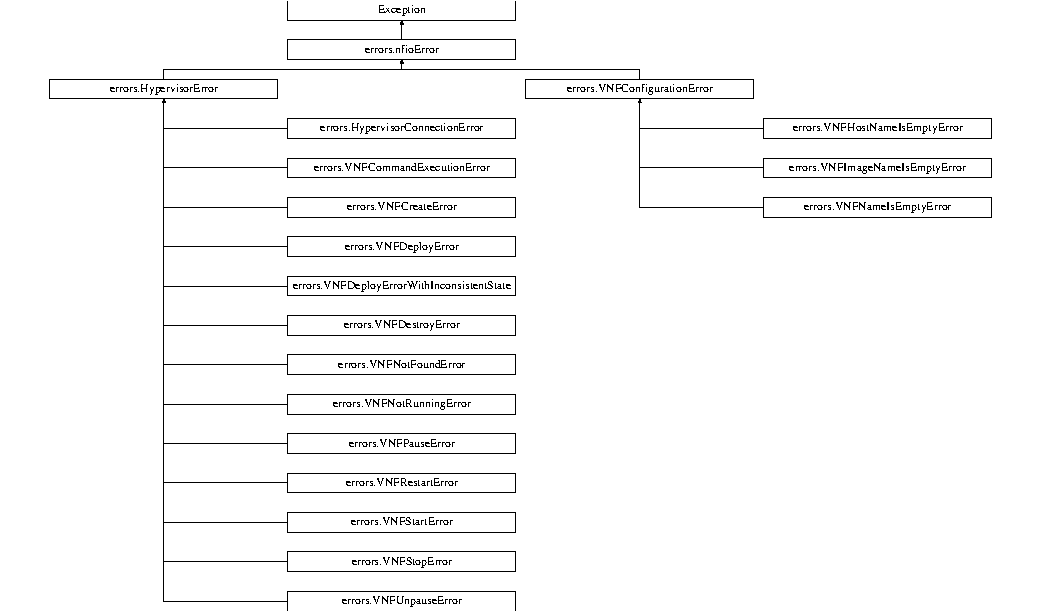
\includegraphics[height=8.205128cm]{classerrors_1_1nfioError}
\end{center}
\end{figure}


\subsection{Detailed Description}
This module contains all the custom exceptions defined for nf.\-io. 

The documentation for this class was generated from the following file\-:\begin{DoxyCompactItemize}
\item 
Wat\-N\-F\-V/nf.\-io/src/errors.\-py\end{DoxyCompactItemize}

\hypertarget{classerrors_1_1VNFCommandExecutionError}{\section{errors.\-V\-N\-F\-Command\-Execution\-Error Class Reference}
\label{classerrors_1_1VNFCommandExecutionError}\index{errors.\-V\-N\-F\-Command\-Execution\-Error@{errors.\-V\-N\-F\-Command\-Execution\-Error}}
}
Inheritance diagram for errors.\-V\-N\-F\-Command\-Execution\-Error\-:\begin{figure}[H]
\begin{center}
\leavevmode
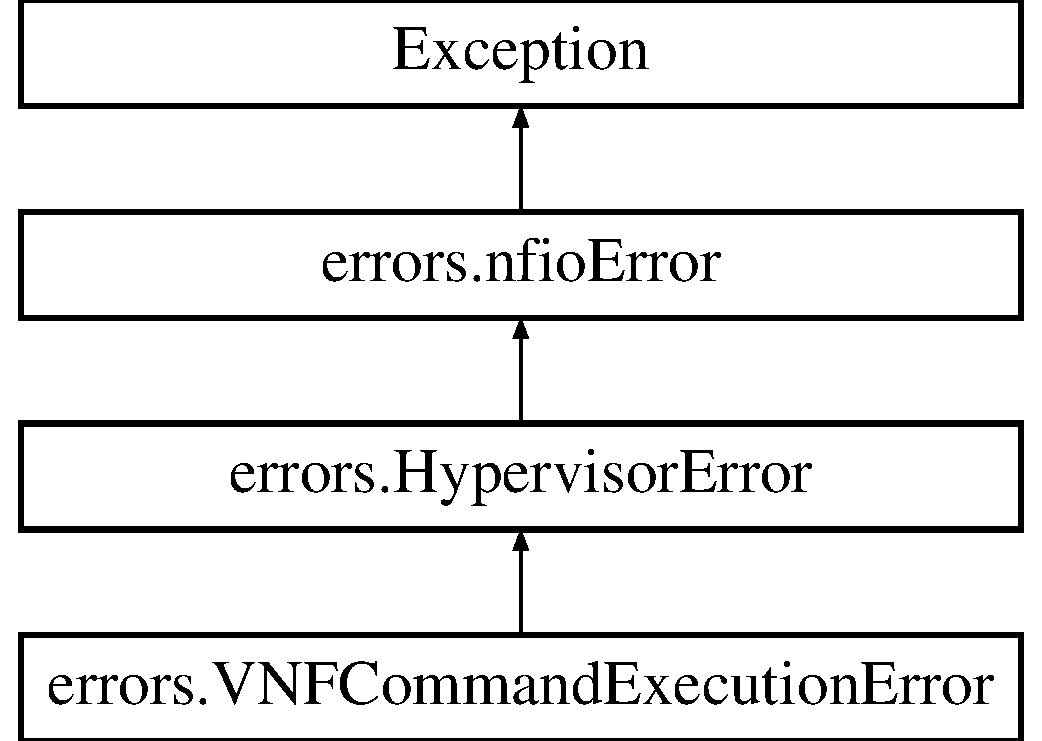
\includegraphics[height=4.000000cm]{classerrors_1_1VNFCommandExecutionError}
\end{center}
\end{figure}
\subsection*{Public Member Functions}
\begin{DoxyCompactItemize}
\item 
\hypertarget{classerrors_1_1VNFCommandExecutionError_af0c11e6123bad9731ea4a2f26a355386}{def {\bfseries \-\_\-\-\_\-init\-\_\-\-\_\-}}\label{classerrors_1_1VNFCommandExecutionError_af0c11e6123bad9731ea4a2f26a355386}

\end{DoxyCompactItemize}
\subsection*{Public Attributes}
\begin{DoxyCompactItemize}
\item 
\hypertarget{classerrors_1_1VNFCommandExecutionError_aaa61a3add5b9a67e6e6076b30d58d2ad}{{\bfseries errno}}\label{classerrors_1_1VNFCommandExecutionError_aaa61a3add5b9a67e6e6076b30d58d2ad}

\end{DoxyCompactItemize}


The documentation for this class was generated from the following file\-:\begin{DoxyCompactItemize}
\item 
Wat\-N\-F\-V/nf.\-io/src/errors.\-py\end{DoxyCompactItemize}

\hypertarget{classerrors_1_1VNFConfigurationError}{\section{errors.\-V\-N\-F\-Configuration\-Error Class Reference}
\label{classerrors_1_1VNFConfigurationError}\index{errors.\-V\-N\-F\-Configuration\-Error@{errors.\-V\-N\-F\-Configuration\-Error}}
}
Inheritance diagram for errors.\-V\-N\-F\-Configuration\-Error\-:\begin{figure}[H]
\begin{center}
\leavevmode
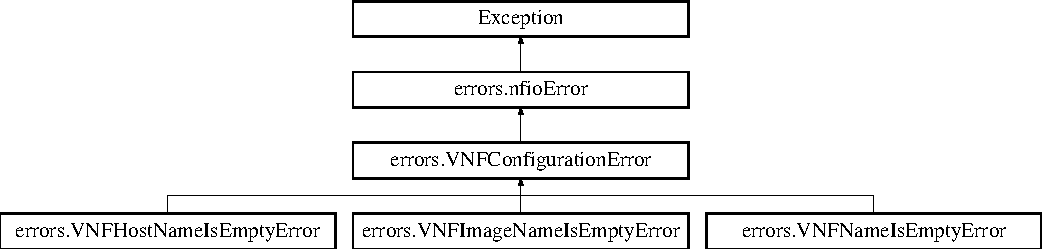
\includegraphics[height=3.348281cm]{classerrors_1_1VNFConfigurationError}
\end{center}
\end{figure}


The documentation for this class was generated from the following file\-:\begin{DoxyCompactItemize}
\item 
Wat\-N\-F\-V/nf.\-io/src/errors.\-py\end{DoxyCompactItemize}

\hypertarget{classerrors_1_1VNFCreateError}{\section{errors.\-V\-N\-F\-Create\-Error Class Reference}
\label{classerrors_1_1VNFCreateError}\index{errors.\-V\-N\-F\-Create\-Error@{errors.\-V\-N\-F\-Create\-Error}}
}
Inheritance diagram for errors.\-V\-N\-F\-Create\-Error\-:\begin{figure}[H]
\begin{center}
\leavevmode
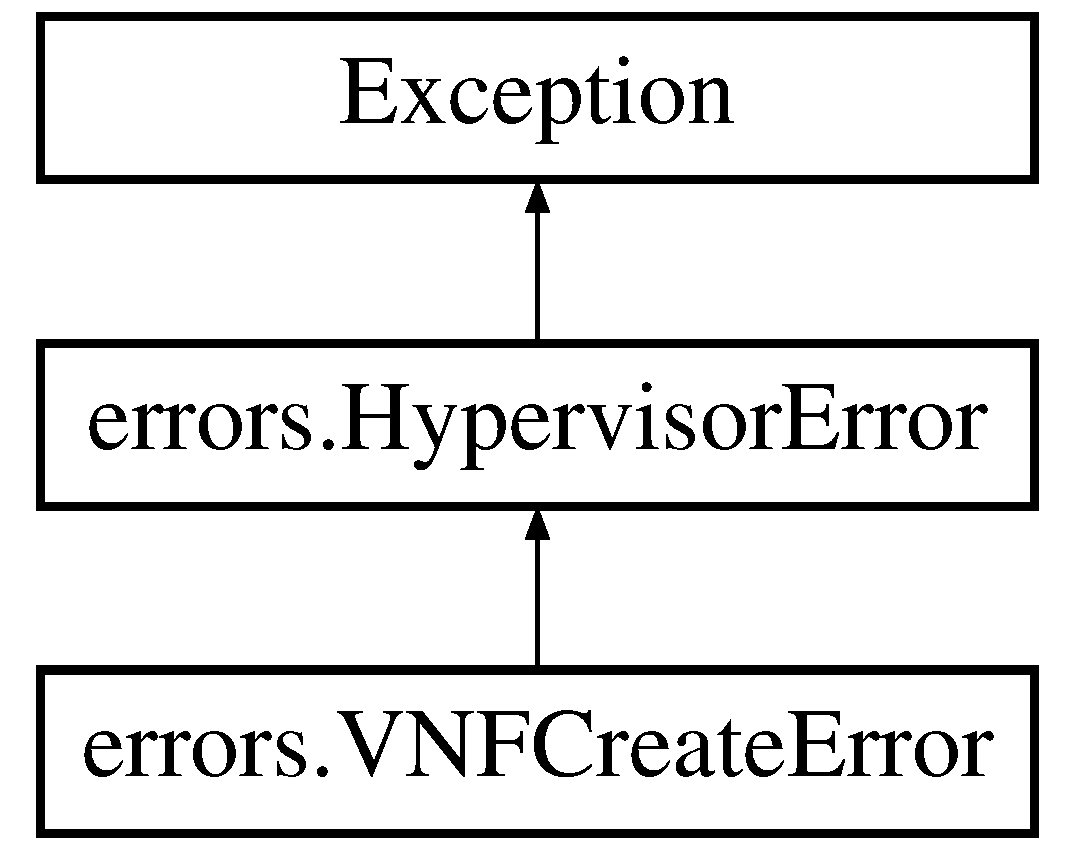
\includegraphics[height=4.000000cm]{classerrors_1_1VNFCreateError}
\end{center}
\end{figure}
\subsection*{Public Member Functions}
\begin{DoxyCompactItemize}
\item 
\hypertarget{classerrors_1_1VNFCreateError_ab23a6006da644303d74177322b2dda27}{def {\bfseries \-\_\-\-\_\-init\-\_\-\-\_\-}}\label{classerrors_1_1VNFCreateError_ab23a6006da644303d74177322b2dda27}

\end{DoxyCompactItemize}
\subsection*{Public Attributes}
\begin{DoxyCompactItemize}
\item 
\hypertarget{classerrors_1_1VNFCreateError_ae18f480a2baf26f11e0b7c37db441930}{{\bfseries errno}}\label{classerrors_1_1VNFCreateError_ae18f480a2baf26f11e0b7c37db441930}

\end{DoxyCompactItemize}


The documentation for this class was generated from the following file\-:\begin{DoxyCompactItemize}
\item 
Wat\-N\-F\-V/nf.\-io/src/errors.\-py\end{DoxyCompactItemize}

\hypertarget{classerrors_1_1VNFDeployError}{\section{errors.\-V\-N\-F\-Deploy\-Error Class Reference}
\label{classerrors_1_1VNFDeployError}\index{errors.\-V\-N\-F\-Deploy\-Error@{errors.\-V\-N\-F\-Deploy\-Error}}
}
Inheritance diagram for errors.\-V\-N\-F\-Deploy\-Error\-:\begin{figure}[H]
\begin{center}
\leavevmode
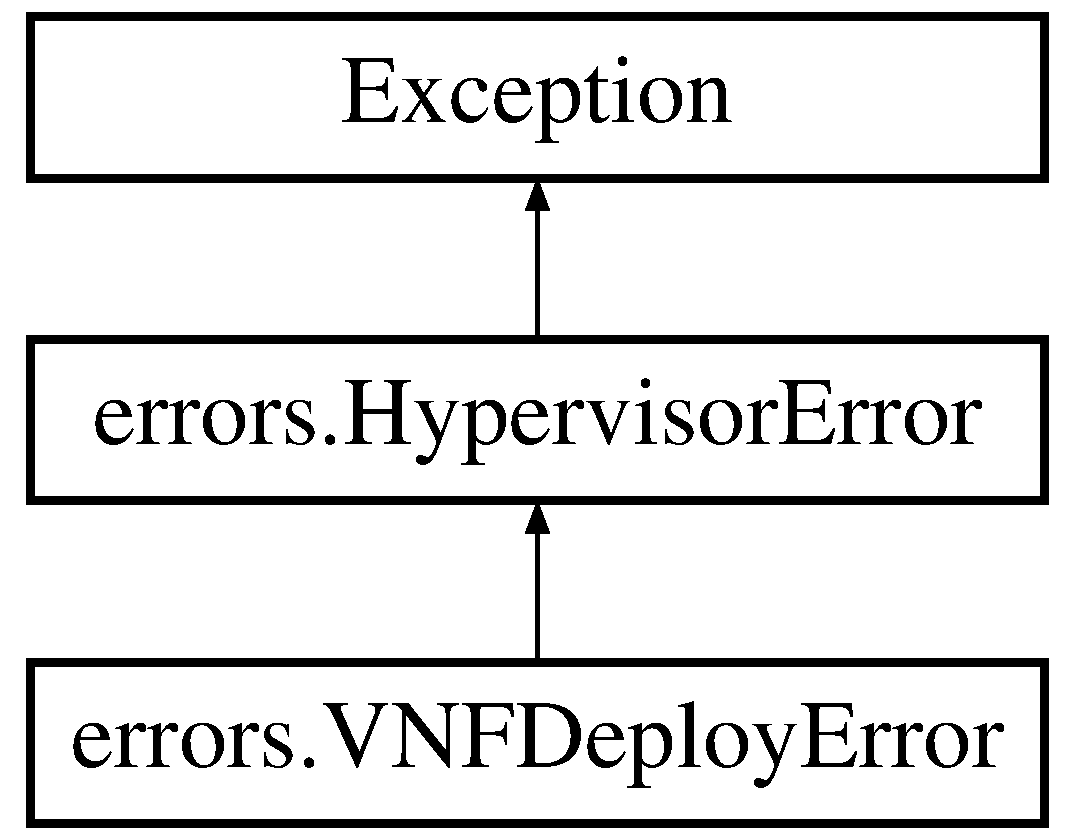
\includegraphics[height=3.000000cm]{classerrors_1_1VNFDeployError}
\end{center}
\end{figure}


The documentation for this class was generated from the following file\-:\begin{DoxyCompactItemize}
\item 
/home/nfuser/nf.\-io/src/errors.\-py\end{DoxyCompactItemize}

\hypertarget{classerrors_1_1VNFDeployErrorWithInconsistentState}{\section{errors.\-V\-N\-F\-Deploy\-Error\-With\-Inconsistent\-State Class Reference}
\label{classerrors_1_1VNFDeployErrorWithInconsistentState}\index{errors.\-V\-N\-F\-Deploy\-Error\-With\-Inconsistent\-State@{errors.\-V\-N\-F\-Deploy\-Error\-With\-Inconsistent\-State}}
}
Inheritance diagram for errors.\-V\-N\-F\-Deploy\-Error\-With\-Inconsistent\-State\-:\begin{figure}[H]
\begin{center}
\leavevmode
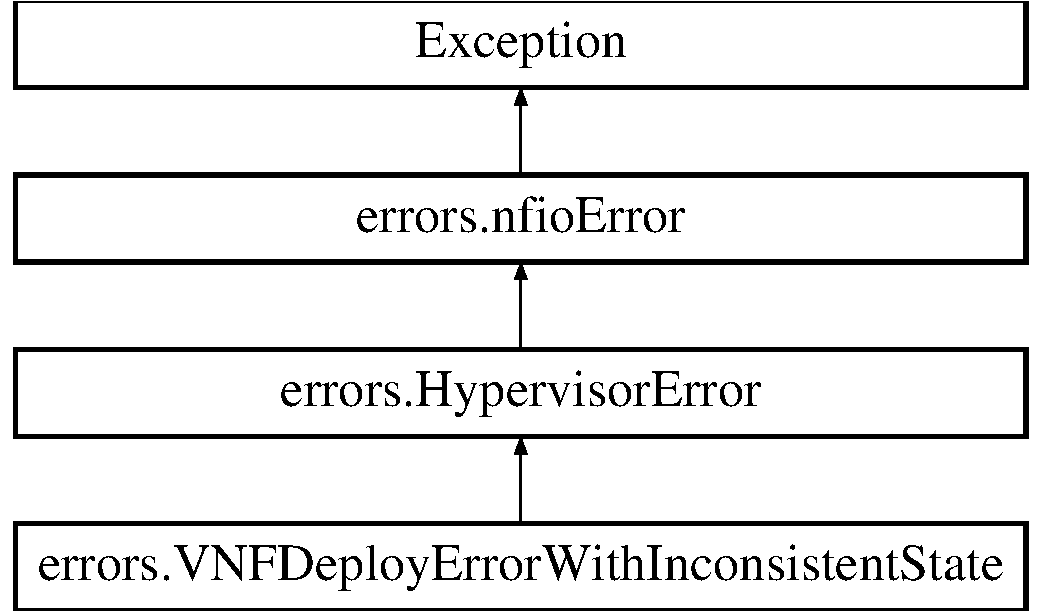
\includegraphics[height=4.000000cm]{classerrors_1_1VNFDeployErrorWithInconsistentState}
\end{center}
\end{figure}
\subsection*{Public Member Functions}
\begin{DoxyCompactItemize}
\item 
\hypertarget{classerrors_1_1VNFDeployErrorWithInconsistentState_a9b0a39ff4609e26174942323865fb6a3}{def {\bfseries \-\_\-\-\_\-init\-\_\-\-\_\-}}\label{classerrors_1_1VNFDeployErrorWithInconsistentState_a9b0a39ff4609e26174942323865fb6a3}

\end{DoxyCompactItemize}
\subsection*{Public Attributes}
\begin{DoxyCompactItemize}
\item 
\hypertarget{classerrors_1_1VNFDeployErrorWithInconsistentState_ae4ac3cc6887b7e1483a209649d18d4b0}{{\bfseries errno}}\label{classerrors_1_1VNFDeployErrorWithInconsistentState_ae4ac3cc6887b7e1483a209649d18d4b0}

\end{DoxyCompactItemize}


\subsection{Detailed Description}


Definition at line 59 of file errors.\-py.



The documentation for this class was generated from the following file\-:\begin{DoxyCompactItemize}
\item 
Wat\-N\-F\-V/nf.\-io/src/errors.\-py\end{DoxyCompactItemize}

\hypertarget{classerrors_1_1VNFDestroyError}{\section{errors.\-V\-N\-F\-Destroy\-Error Class Reference}
\label{classerrors_1_1VNFDestroyError}\index{errors.\-V\-N\-F\-Destroy\-Error@{errors.\-V\-N\-F\-Destroy\-Error}}
}
Inheritance diagram for errors.\-V\-N\-F\-Destroy\-Error\-:\begin{figure}[H]
\begin{center}
\leavevmode
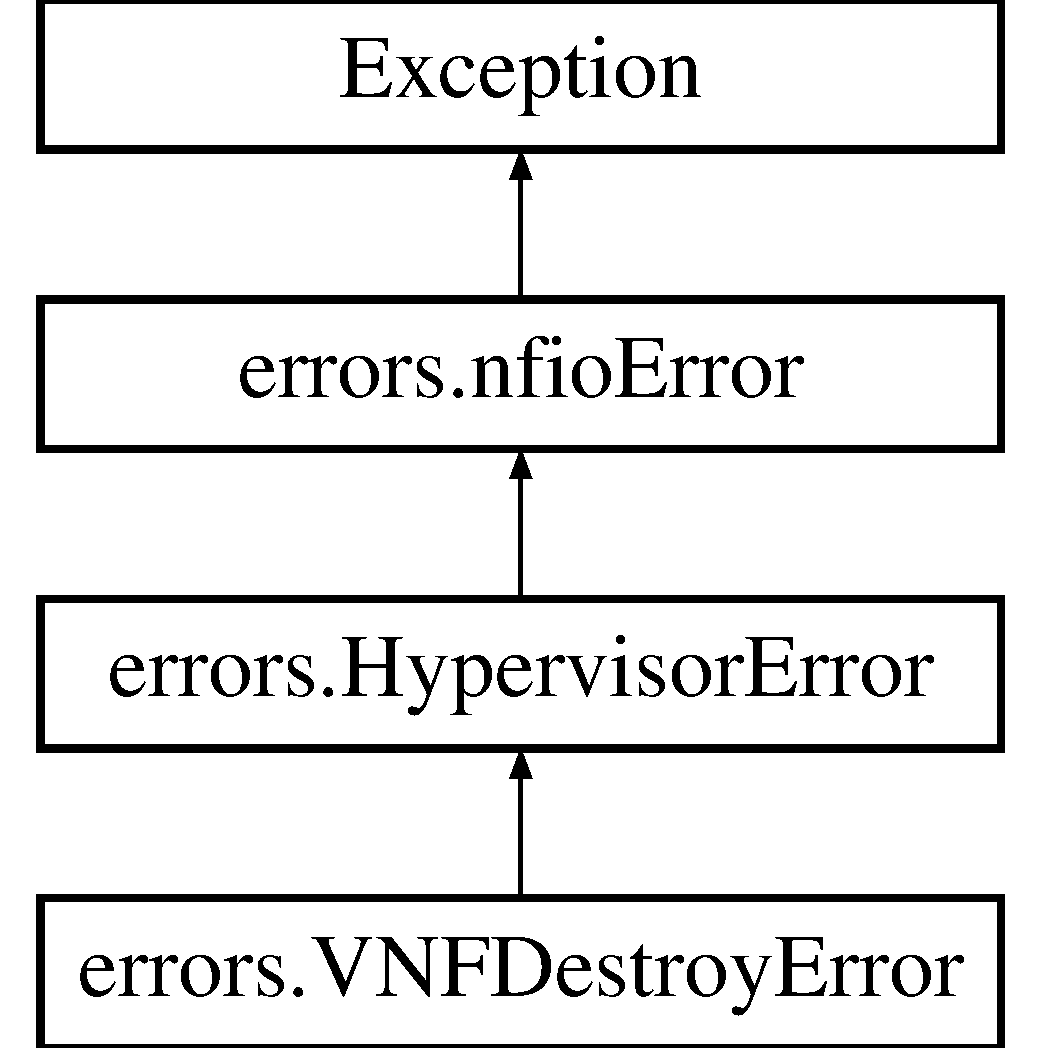
\includegraphics[height=3.000000cm]{classerrors_1_1VNFDestroyError}
\end{center}
\end{figure}


The documentation for this class was generated from the following file\-:\begin{DoxyCompactItemize}
\item 
/home/nfuser/nf.\-io/src/errors.\-py\end{DoxyCompactItemize}

\hypertarget{classerrors_1_1VNFHostNameIsEmptyError}{\section{errors.\-V\-N\-F\-Host\-Name\-Is\-Empty\-Error Class Reference}
\label{classerrors_1_1VNFHostNameIsEmptyError}\index{errors.\-V\-N\-F\-Host\-Name\-Is\-Empty\-Error@{errors.\-V\-N\-F\-Host\-Name\-Is\-Empty\-Error}}
}
Inheritance diagram for errors.\-V\-N\-F\-Host\-Name\-Is\-Empty\-Error\-:\begin{figure}[H]
\begin{center}
\leavevmode
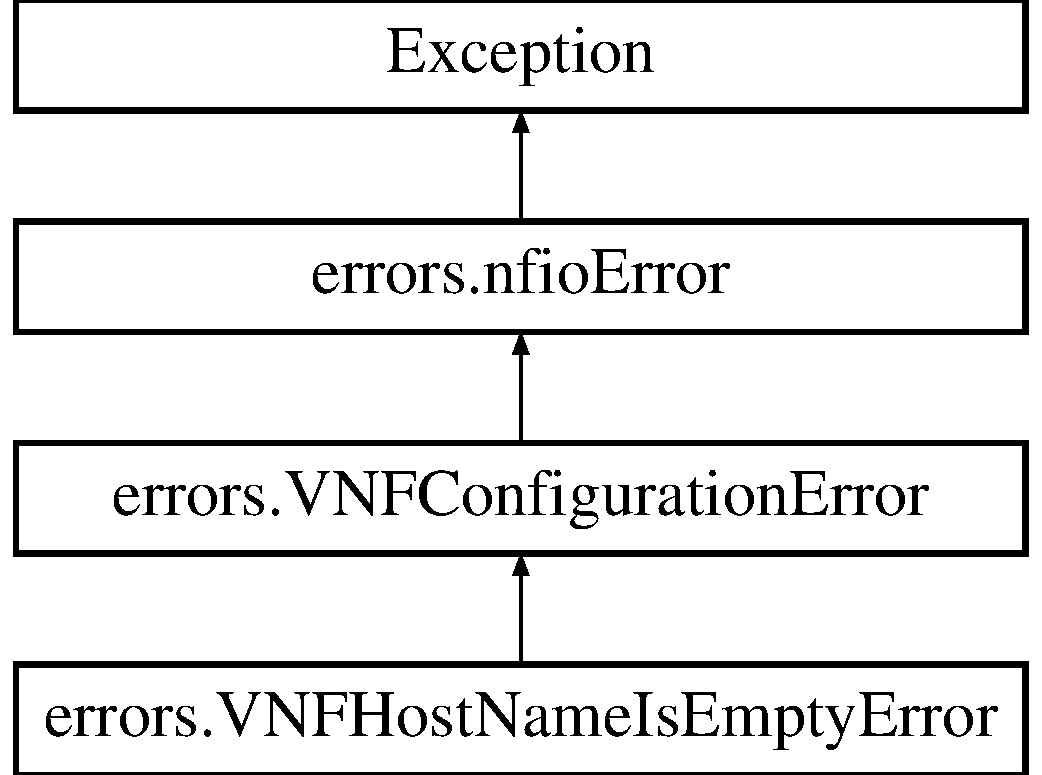
\includegraphics[height=4.000000cm]{classerrors_1_1VNFHostNameIsEmptyError}
\end{center}
\end{figure}
\subsection*{Public Member Functions}
\begin{DoxyCompactItemize}
\item 
\hypertarget{classerrors_1_1VNFHostNameIsEmptyError_a54ff177a72b031db9662672cbc262f86}{def {\bfseries \-\_\-\-\_\-init\-\_\-\-\_\-}}\label{classerrors_1_1VNFHostNameIsEmptyError_a54ff177a72b031db9662672cbc262f86}

\end{DoxyCompactItemize}
\subsection*{Public Attributes}
\begin{DoxyCompactItemize}
\item 
\hypertarget{classerrors_1_1VNFHostNameIsEmptyError_a4a67c7308f0dede292cf6b5654324f39}{{\bfseries errno}}\label{classerrors_1_1VNFHostNameIsEmptyError_a4a67c7308f0dede292cf6b5654324f39}

\end{DoxyCompactItemize}


The documentation for this class was generated from the following file\-:\begin{DoxyCompactItemize}
\item 
Wat\-N\-F\-V/nf.\-io/src/errors.\-py\end{DoxyCompactItemize}

\hypertarget{classerrors_1_1VNFImageNameIsEmptyError}{\section{errors.\-V\-N\-F\-Image\-Name\-Is\-Empty\-Error Class Reference}
\label{classerrors_1_1VNFImageNameIsEmptyError}\index{errors.\-V\-N\-F\-Image\-Name\-Is\-Empty\-Error@{errors.\-V\-N\-F\-Image\-Name\-Is\-Empty\-Error}}
}
Inheritance diagram for errors.\-V\-N\-F\-Image\-Name\-Is\-Empty\-Error\-:\begin{figure}[H]
\begin{center}
\leavevmode
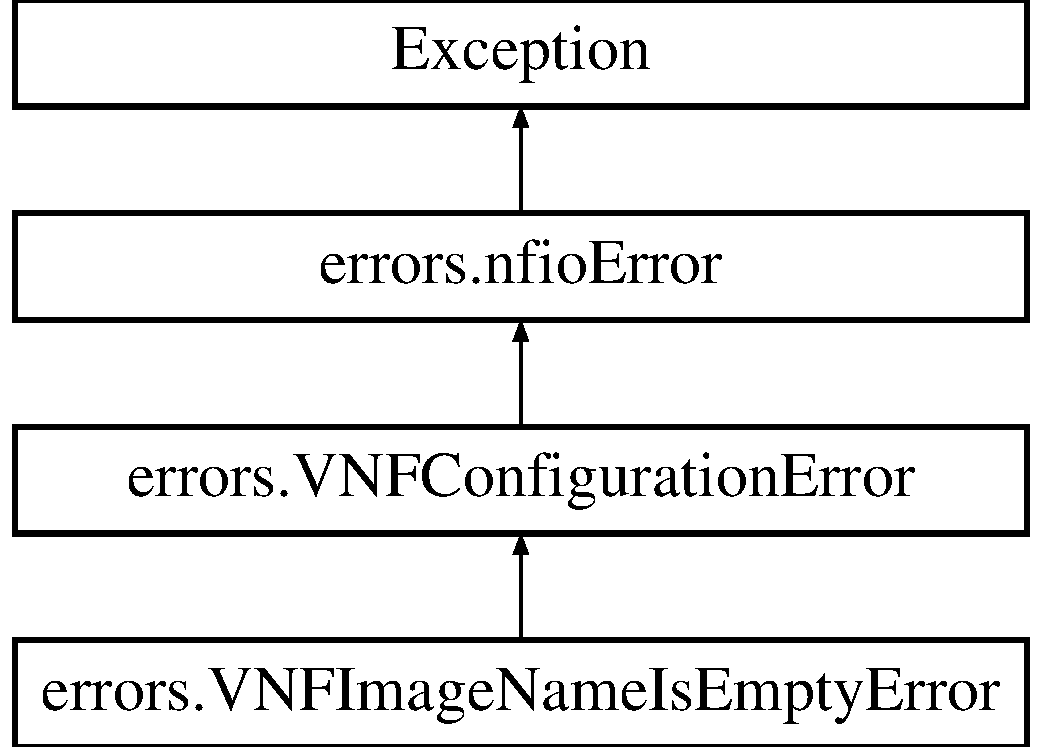
\includegraphics[height=4.000000cm]{classerrors_1_1VNFImageNameIsEmptyError}
\end{center}
\end{figure}
\subsection*{Public Member Functions}
\begin{DoxyCompactItemize}
\item 
\hypertarget{classerrors_1_1VNFImageNameIsEmptyError_a58a6d457d974dd896fa1d9f3db0392ed}{def {\bfseries \-\_\-\-\_\-init\-\_\-\-\_\-}}\label{classerrors_1_1VNFImageNameIsEmptyError_a58a6d457d974dd896fa1d9f3db0392ed}

\end{DoxyCompactItemize}
\subsection*{Public Attributes}
\begin{DoxyCompactItemize}
\item 
\hypertarget{classerrors_1_1VNFImageNameIsEmptyError_a51eb42467bf171acfba9c993e378580b}{{\bfseries errno}}\label{classerrors_1_1VNFImageNameIsEmptyError_a51eb42467bf171acfba9c993e378580b}

\end{DoxyCompactItemize}


The documentation for this class was generated from the following file\-:\begin{DoxyCompactItemize}
\item 
Wat\-N\-F\-V/nf.\-io/src/errors.\-py\end{DoxyCompactItemize}

\hypertarget{classerrors_1_1VNFNameIsEmptyError}{\section{errors.\-V\-N\-F\-Name\-Is\-Empty\-Error Class Reference}
\label{classerrors_1_1VNFNameIsEmptyError}\index{errors.\-V\-N\-F\-Name\-Is\-Empty\-Error@{errors.\-V\-N\-F\-Name\-Is\-Empty\-Error}}
}
Inheritance diagram for errors.\-V\-N\-F\-Name\-Is\-Empty\-Error\-:\begin{figure}[H]
\begin{center}
\leavevmode
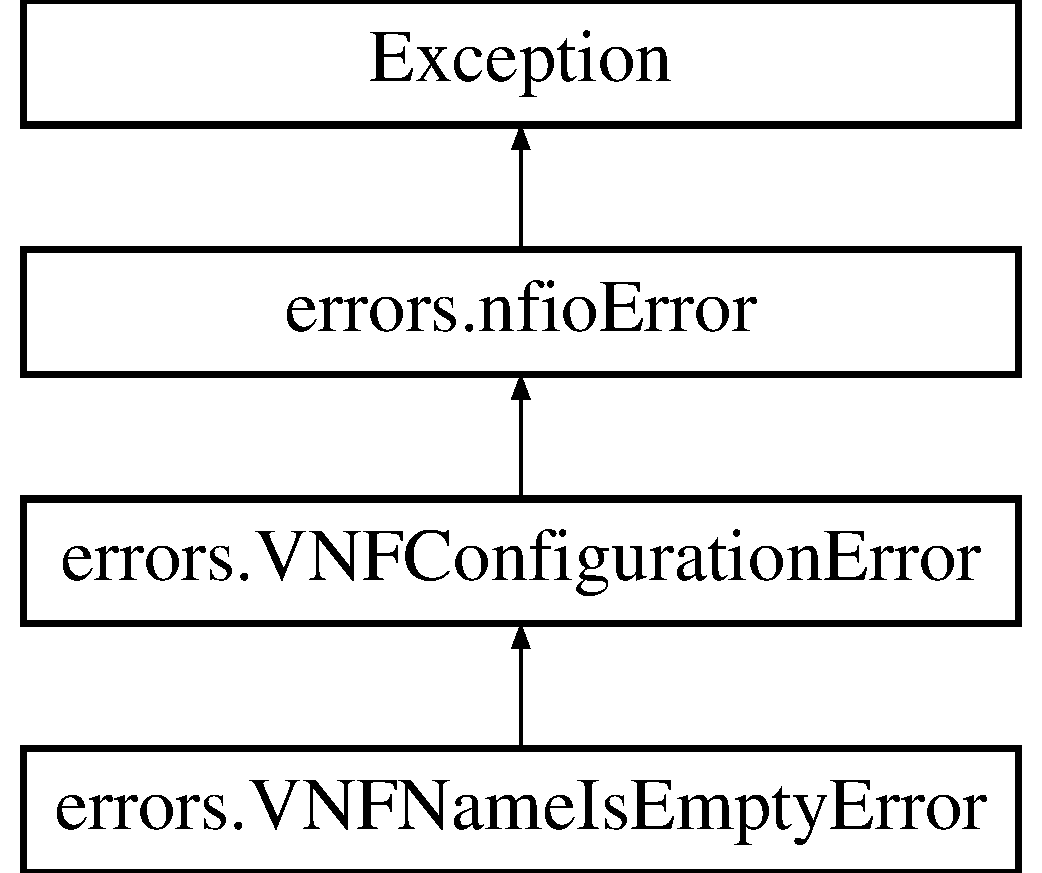
\includegraphics[height=4.000000cm]{classerrors_1_1VNFNameIsEmptyError}
\end{center}
\end{figure}
\subsection*{Public Member Functions}
\begin{DoxyCompactItemize}
\item 
\hypertarget{classerrors_1_1VNFNameIsEmptyError_ae551ab48dee839aa8e2a35b43801e1f9}{def {\bfseries \-\_\-\-\_\-init\-\_\-\-\_\-}}\label{classerrors_1_1VNFNameIsEmptyError_ae551ab48dee839aa8e2a35b43801e1f9}

\end{DoxyCompactItemize}
\subsection*{Public Attributes}
\begin{DoxyCompactItemize}
\item 
\hypertarget{classerrors_1_1VNFNameIsEmptyError_a6c69f18aa91b91ffb8b2483d1e1c4dba}{{\bfseries errno}}\label{classerrors_1_1VNFNameIsEmptyError_a6c69f18aa91b91ffb8b2483d1e1c4dba}

\end{DoxyCompactItemize}


The documentation for this class was generated from the following file\-:\begin{DoxyCompactItemize}
\item 
Wat\-N\-F\-V/nf.\-io/src/errors.\-py\end{DoxyCompactItemize}

\hypertarget{classerrors_1_1VNFNotFoundError}{\section{errors.\-V\-N\-F\-Not\-Found\-Error Class Reference}
\label{classerrors_1_1VNFNotFoundError}\index{errors.\-V\-N\-F\-Not\-Found\-Error@{errors.\-V\-N\-F\-Not\-Found\-Error}}
}
Inheritance diagram for errors.\-V\-N\-F\-Not\-Found\-Error\-:\begin{figure}[H]
\begin{center}
\leavevmode
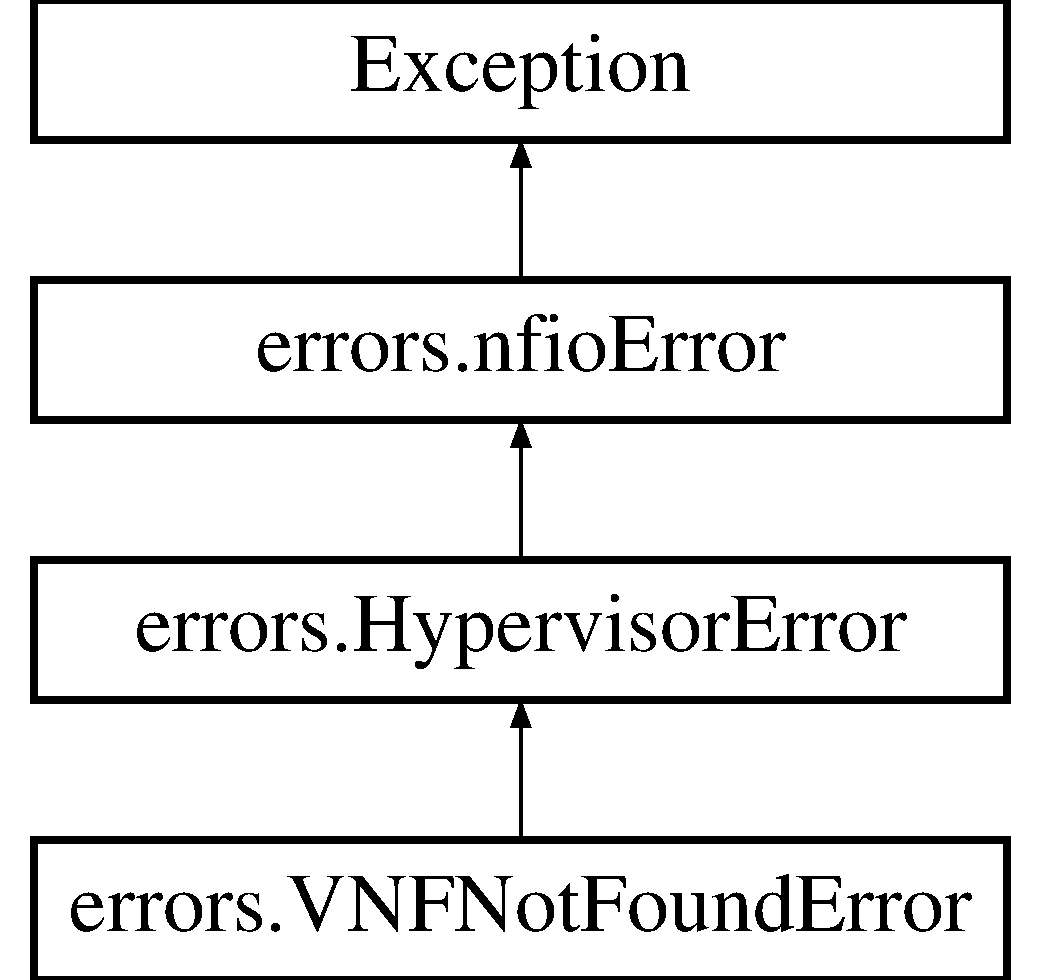
\includegraphics[height=4.000000cm]{classerrors_1_1VNFNotFoundError}
\end{center}
\end{figure}
\subsection*{Public Member Functions}
\begin{DoxyCompactItemize}
\item 
\hypertarget{classerrors_1_1VNFNotFoundError_a929f3afe0fed32e5a0d345fed81583ba}{def {\bfseries \-\_\-\-\_\-init\-\_\-\-\_\-}}\label{classerrors_1_1VNFNotFoundError_a929f3afe0fed32e5a0d345fed81583ba}

\end{DoxyCompactItemize}
\subsection*{Public Attributes}
\begin{DoxyCompactItemize}
\item 
\hypertarget{classerrors_1_1VNFNotFoundError_a972c73f0a6d8a4f4f4abbb54b4da9df5}{{\bfseries errno}}\label{classerrors_1_1VNFNotFoundError_a972c73f0a6d8a4f4f4abbb54b4da9df5}

\end{DoxyCompactItemize}


\subsection{Detailed Description}


Definition at line 19 of file errors.\-py.



The documentation for this class was generated from the following file\-:\begin{DoxyCompactItemize}
\item 
Wat\-N\-F\-V/nf.\-io/src/errors.\-py\end{DoxyCompactItemize}

\hypertarget{classerrors_1_1VNFNotRunningError}{\section{errors.\-V\-N\-F\-Not\-Running\-Error Class Reference}
\label{classerrors_1_1VNFNotRunningError}\index{errors.\-V\-N\-F\-Not\-Running\-Error@{errors.\-V\-N\-F\-Not\-Running\-Error}}
}
Inheritance diagram for errors.\-V\-N\-F\-Not\-Running\-Error\-:\begin{figure}[H]
\begin{center}
\leavevmode
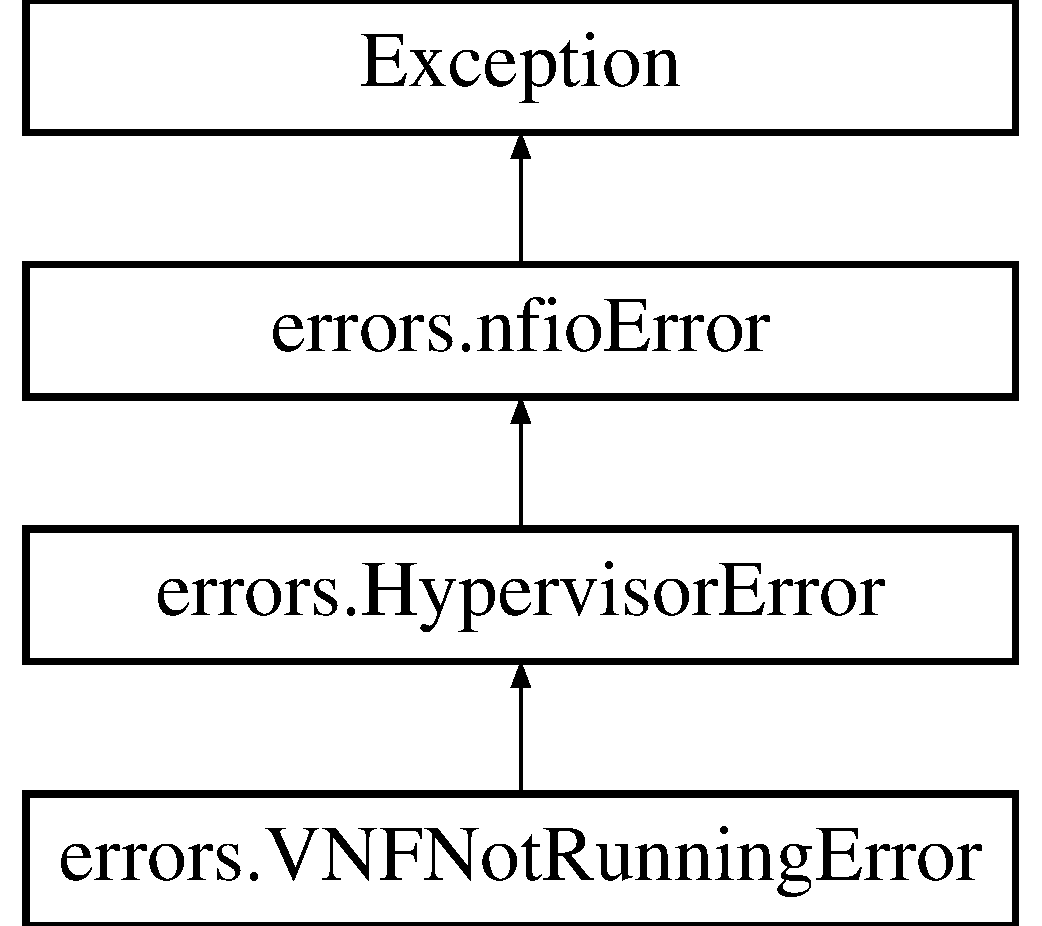
\includegraphics[height=4.000000cm]{classerrors_1_1VNFNotRunningError}
\end{center}
\end{figure}
\subsection*{Public Member Functions}
\begin{DoxyCompactItemize}
\item 
\hypertarget{classerrors_1_1VNFNotRunningError_a9f548d7d752d002aad923fa0d39a9e12}{def {\bfseries \-\_\-\-\_\-init\-\_\-\-\_\-}}\label{classerrors_1_1VNFNotRunningError_a9f548d7d752d002aad923fa0d39a9e12}

\end{DoxyCompactItemize}
\subsection*{Public Attributes}
\begin{DoxyCompactItemize}
\item 
\hypertarget{classerrors_1_1VNFNotRunningError_a0851579bdfdaf110fa92e6d2df503827}{{\bfseries errno}}\label{classerrors_1_1VNFNotRunningError_a0851579bdfdaf110fa92e6d2df503827}

\end{DoxyCompactItemize}


The documentation for this class was generated from the following file\-:\begin{DoxyCompactItemize}
\item 
Wat\-N\-F\-V/nf.\-io/src/errors.\-py\end{DoxyCompactItemize}

\hypertarget{classerrors_1_1VNFPauseError}{\section{errors.\-V\-N\-F\-Pause\-Error Class Reference}
\label{classerrors_1_1VNFPauseError}\index{errors.\-V\-N\-F\-Pause\-Error@{errors.\-V\-N\-F\-Pause\-Error}}
}
Inheritance diagram for errors.\-V\-N\-F\-Pause\-Error\-:\begin{figure}[H]
\begin{center}
\leavevmode
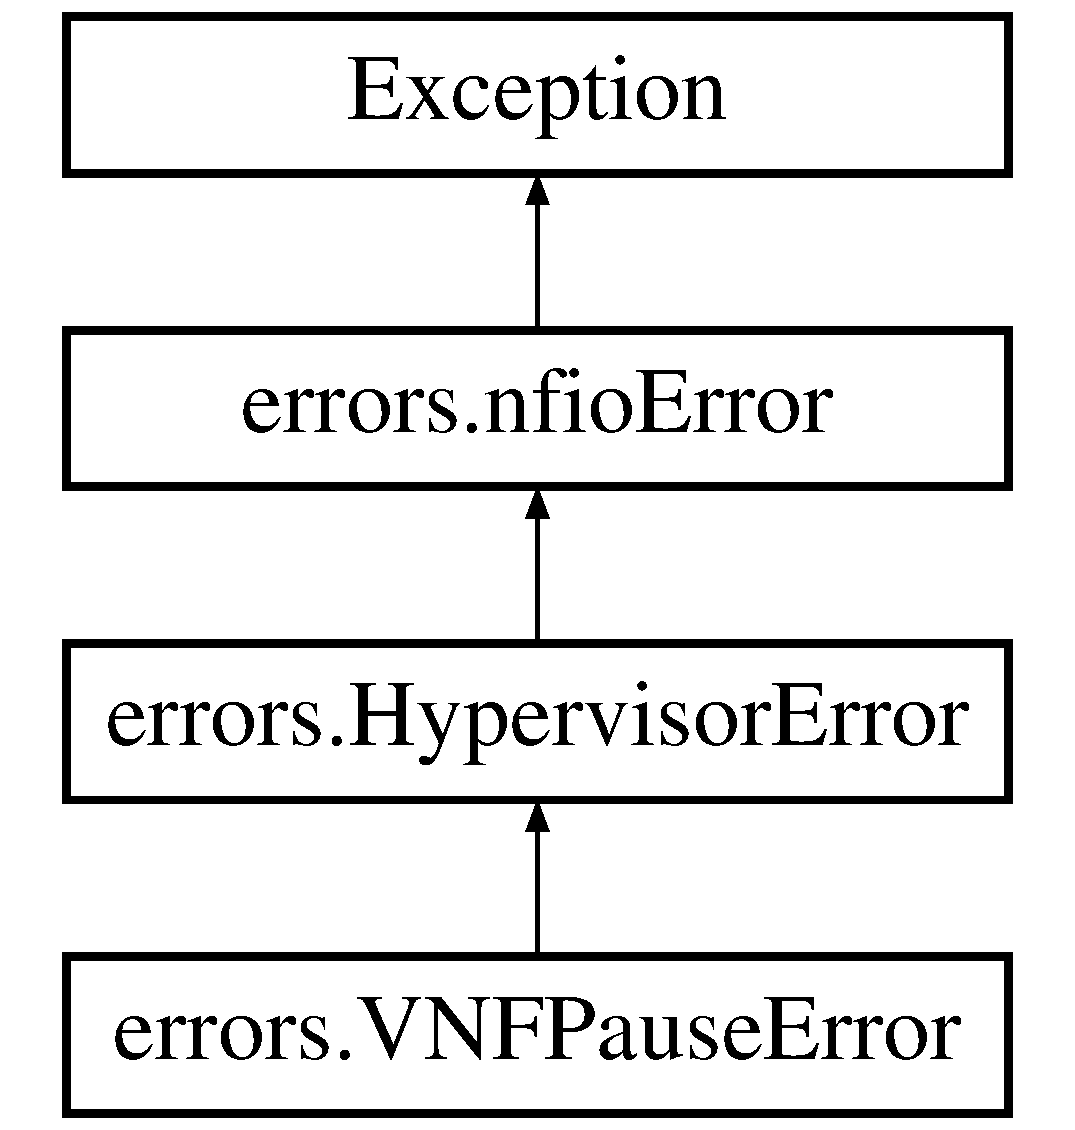
\includegraphics[height=4.000000cm]{classerrors_1_1VNFPauseError}
\end{center}
\end{figure}
\subsection*{Public Member Functions}
\begin{DoxyCompactItemize}
\item 
\hypertarget{classerrors_1_1VNFPauseError_af180dd953405832564b68629f76c0de2}{def {\bfseries \-\_\-\-\_\-init\-\_\-\-\_\-}}\label{classerrors_1_1VNFPauseError_af180dd953405832564b68629f76c0de2}

\end{DoxyCompactItemize}
\subsection*{Public Attributes}
\begin{DoxyCompactItemize}
\item 
\hypertarget{classerrors_1_1VNFPauseError_a410926f683c51832b1e9339b2acf8069}{{\bfseries errno}}\label{classerrors_1_1VNFPauseError_a410926f683c51832b1e9339b2acf8069}

\end{DoxyCompactItemize}


The documentation for this class was generated from the following file\-:\begin{DoxyCompactItemize}
\item 
Wat\-N\-F\-V/nf.\-io/src/errors.\-py\end{DoxyCompactItemize}

\hypertarget{classerrors_1_1VNFRestartError}{\section{errors.\-V\-N\-F\-Restart\-Error Class Reference}
\label{classerrors_1_1VNFRestartError}\index{errors.\-V\-N\-F\-Restart\-Error@{errors.\-V\-N\-F\-Restart\-Error}}
}
Inheritance diagram for errors.\-V\-N\-F\-Restart\-Error\-:\begin{figure}[H]
\begin{center}
\leavevmode
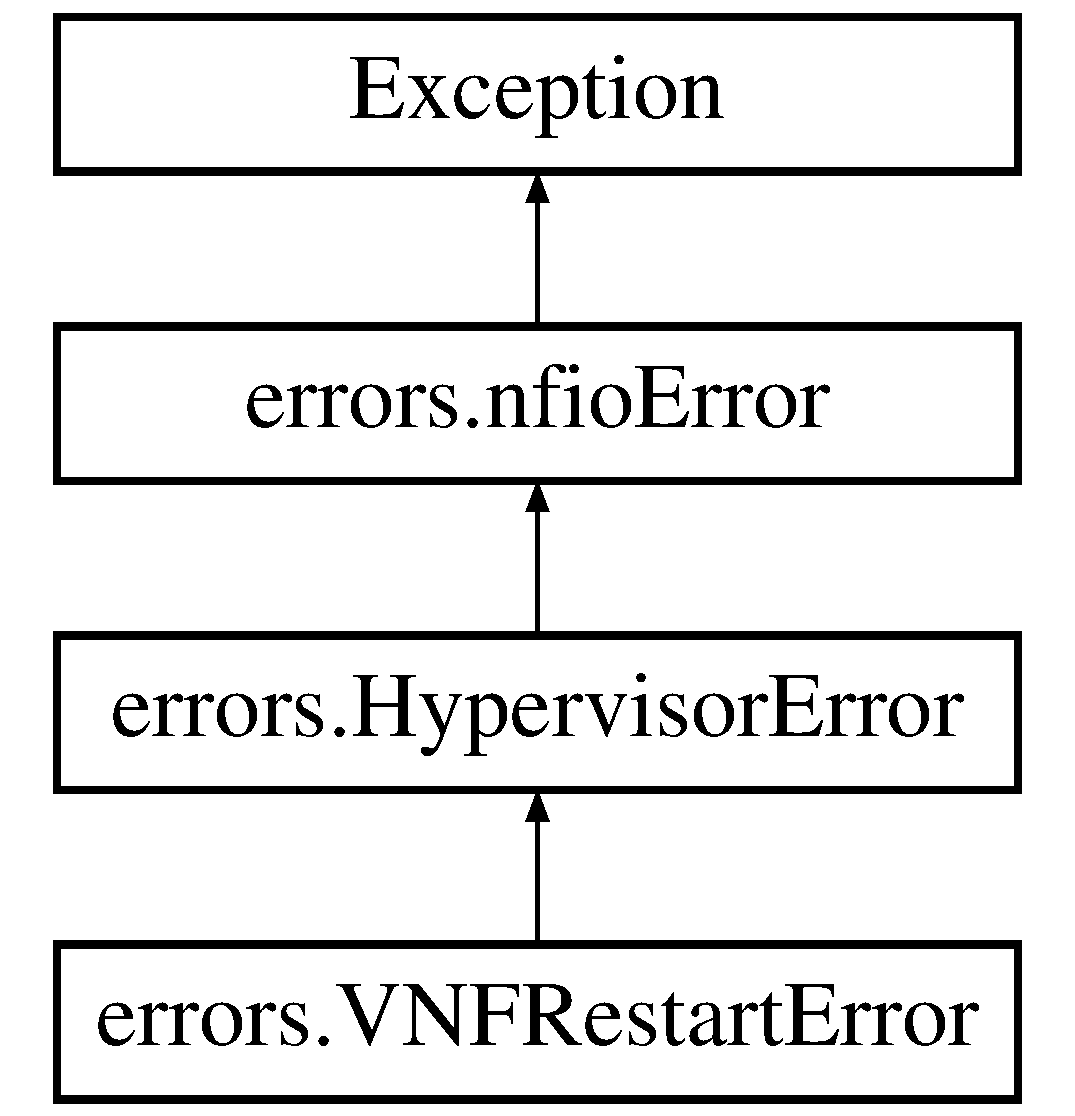
\includegraphics[height=3.000000cm]{classerrors_1_1VNFRestartError}
\end{center}
\end{figure}


The documentation for this class was generated from the following file\-:\begin{DoxyCompactItemize}
\item 
/home/nfuser/nf.\-io/src/errors.\-py\end{DoxyCompactItemize}

\hypertarget{classvnfs__operations_1_1VNFSOperations}{\section{vnfs\-\_\-operations.\-V\-N\-F\-S\-Operations Class Reference}
\label{classvnfs__operations_1_1VNFSOperations}\index{vnfs\-\_\-operations.\-V\-N\-F\-S\-Operations@{vnfs\-\_\-operations.\-V\-N\-F\-S\-Operations}}
}


Provides a common set of operations for nfio.  


\subsection*{Public Member Functions}
\begin{DoxyCompactItemize}
\item 
\hypertarget{classvnfs__operations_1_1VNFSOperations_a8aeb0c031c7f7b97e8544ed7d8c49b35}{def {\bfseries \-\_\-\-\_\-init\-\_\-\-\_\-}}\label{classvnfs__operations_1_1VNFSOperations_a8aeb0c031c7f7b97e8544ed7d8c49b35}

\item 
def \hyperlink{classvnfs__operations_1_1VNFSOperations_ae73c421b301cbda862896f9fe67a7941}{vnfs\-\_\-create\-\_\-vnf\-\_\-instance}
\begin{DoxyCompactList}\small\item\em Create the file system structure for a V\-N\-F. \end{DoxyCompactList}\item 
def \hyperlink{classvnfs__operations_1_1VNFSOperations_a3c0b706c40d09a2ed679aed33d37b5e9}{vnfs\-\_\-get\-\_\-opcode}
\begin{DoxyCompactList}\small\item\em Determinse the type of operation based on the path. \end{DoxyCompactList}\item 
def \hyperlink{classvnfs__operations_1_1VNFSOperations_a75430767bdb54f256059c588058b3323}{vnfs\-\_\-get\-\_\-nf\-\_\-type}
\begin{DoxyCompactList}\small\item\em Parse the type of V\-N\-F from path. \end{DoxyCompactList}\item 
def \hyperlink{classvnfs__operations_1_1VNFSOperations_a9461289b4af0fef0db381e5ec17a6cac}{vnfs\-\_\-get\-\_\-file\-\_\-name}
\begin{DoxyCompactList}\small\item\em Return the name of the file represented by a path. \end{DoxyCompactList}\item 
def \hyperlink{classvnfs__operations_1_1VNFSOperations_a464c0ebd7c574c62d76d352a3a59aec0}{vnfs\-\_\-is\-\_\-nf\-\_\-instance}
\begin{DoxyCompactList}\small\item\em Determines if a path represents an nf instance directory. \end{DoxyCompactList}\item 
def \hyperlink{classvnfs__operations_1_1VNFSOperations_a367f1d6fb6749b0a16af47381d43c874}{vnfs\-\_\-get\-\_\-instance\-\_\-configuration}
\begin{DoxyCompactList}\small\item\em Return the configuration parameters related to a V\-N\-F instance. \end{DoxyCompactList}\item 
def \hyperlink{classvnfs__operations_1_1VNFSOperations_a304bb0780682b050cdf9d43e3f279ead}{vnfs\-\_\-deploy\-\_\-nf}
\begin{DoxyCompactList}\small\item\em Deploys and S\-T\-A\-R\-T\-S a V\-N\-F instance. \end{DoxyCompactList}\item 
def \hyperlink{classvnfs__operations_1_1VNFSOperations_a3c95617427fa157dbde8246a260546ed}{vnfs\-\_\-stop\-\_\-vnf}
\begin{DoxyCompactList}\small\item\em Stops a V\-N\-F instance. \end{DoxyCompactList}\item 
def \hyperlink{classvnfs__operations_1_1VNFSOperations_a1f88fc97d23ebfac8a99a71542ca5219}{vnfs\-\_\-start\-\_\-vnf}
\begin{DoxyCompactList}\small\item\em Starts a deployed V\-N\-F instance. \end{DoxyCompactList}\item 
def \hyperlink{classvnfs__operations_1_1VNFSOperations_a54389b0c8a5a740746816e3c99066685}{vnfs\-\_\-destroy\-\_\-vnf}
\begin{DoxyCompactList}\small\item\em Destroys a deployed V\-N\-F instance. \end{DoxyCompactList}\item 
def \hyperlink{classvnfs__operations_1_1VNFSOperations_a27409856538f49f14a8506635ded95b7}{vnfs\-\_\-get\-\_\-rx\-\_\-bytes}
\begin{DoxyCompactList}\small\item\em Reads the number of bytes received by a V\-N\-F instance. \end{DoxyCompactList}\item 
def \hyperlink{classvnfs__operations_1_1VNFSOperations_ab4617f4573ef7d6c4106b0fdbf728022}{vnfs\-\_\-get\-\_\-tx\-\_\-bytes}
\begin{DoxyCompactList}\small\item\em Reads the number of bytes sent by a V\-N\-F instance. \end{DoxyCompactList}\item 
def \hyperlink{classvnfs__operations_1_1VNFSOperations_a05a7ab8ae7e8a2ab7502a1d4e0113144}{vnfs\-\_\-get\-\_\-pkt\-\_\-drops}
\begin{DoxyCompactList}\small\item\em Reads the number of packets dropped by a V\-N\-F instance. \end{DoxyCompactList}\item 
def \hyperlink{classvnfs__operations_1_1VNFSOperations_ac2787ee33d5944c39a07321e270bdcfd}{vnfs\-\_\-get\-\_\-status}
\begin{DoxyCompactList}\small\item\em Get the status of a V\-N\-F instance, e.\-g., the V\-N\-F is running/suspended/stopped etc. \end{DoxyCompactList}\item 
def \hyperlink{classvnfs__operations_1_1VNFSOperations_a482dc96295584a1ca84300f04d000f26}{vnfs\-\_\-get\-\_\-ip}
\begin{DoxyCompactList}\small\item\em Get the status of a V\-N\-F instance, e.\-g., the V\-N\-F is running/suspended/stopped etc. \end{DoxyCompactList}\end{DoxyCompactItemize}
\subsection*{Public Attributes}
\begin{DoxyCompactItemize}
\item 
\hypertarget{classvnfs__operations_1_1VNFSOperations_a88ae8c710ff0d9f76a72d2da2d736e34}{{\bfseries vnfs\-\_\-root}}\label{classvnfs__operations_1_1VNFSOperations_a88ae8c710ff0d9f76a72d2da2d736e34}

\end{DoxyCompactItemize}
\subsection*{Static Public Attributes}
\begin{DoxyCompactItemize}
\item 
\hypertarget{classvnfs__operations_1_1VNFSOperations_a4477fd75c80184251d2894d71e3dee5e}{int {\bfseries O\-P\-\_\-\-U\-N\-D\-E\-F\-I\-N\-E\-D} = 0x\-F\-F}\label{classvnfs__operations_1_1VNFSOperations_a4477fd75c80184251d2894d71e3dee5e}

\item 
\hypertarget{classvnfs__operations_1_1VNFSOperations_a1cde1da5a03e27b526f1a71e2a6244ff}{int {\bfseries O\-P\-\_\-\-N\-F} = 0x01}\label{classvnfs__operations_1_1VNFSOperations_a1cde1da5a03e27b526f1a71e2a6244ff}

\end{DoxyCompactItemize}


\subsection{Detailed Description}
Provides a common set of operations for nfio. 

These operations act as a helper. 

\subsection{Member Function Documentation}
\hypertarget{classvnfs__operations_1_1VNFSOperations_ae73c421b301cbda862896f9fe67a7941}{\index{vnfs\-\_\-operations\-::\-V\-N\-F\-S\-Operations@{vnfs\-\_\-operations\-::\-V\-N\-F\-S\-Operations}!vnfs\-\_\-create\-\_\-vnf\-\_\-instance@{vnfs\-\_\-create\-\_\-vnf\-\_\-instance}}
\index{vnfs\-\_\-create\-\_\-vnf\-\_\-instance@{vnfs\-\_\-create\-\_\-vnf\-\_\-instance}!vnfs_operations::VNFSOperations@{vnfs\-\_\-operations\-::\-V\-N\-F\-S\-Operations}}
\subsubsection[{vnfs\-\_\-create\-\_\-vnf\-\_\-instance}]{\setlength{\rightskip}{0pt plus 5cm}def vnfs\-\_\-operations.\-V\-N\-F\-S\-Operations.\-vnfs\-\_\-create\-\_\-vnf\-\_\-instance (
\begin{DoxyParamCaption}
\item[{}]{self, }
\item[{}]{path, }
\item[{}]{mode}
\end{DoxyParamCaption}
)}}\label{classvnfs__operations_1_1VNFSOperations_ae73c421b301cbda862896f9fe67a7941}


Create the file system structure for a V\-N\-F. 

Args\-: path\-: path of the new V\-N\-F instance. mode\-: file creation mode for the new V\-N\-F instance directory.

Returns\-: returns the return code of os.\-mkdir \hypertarget{classvnfs__operations_1_1VNFSOperations_a304bb0780682b050cdf9d43e3f279ead}{\index{vnfs\-\_\-operations\-::\-V\-N\-F\-S\-Operations@{vnfs\-\_\-operations\-::\-V\-N\-F\-S\-Operations}!vnfs\-\_\-deploy\-\_\-nf@{vnfs\-\_\-deploy\-\_\-nf}}
\index{vnfs\-\_\-deploy\-\_\-nf@{vnfs\-\_\-deploy\-\_\-nf}!vnfs_operations::VNFSOperations@{vnfs\-\_\-operations\-::\-V\-N\-F\-S\-Operations}}
\subsubsection[{vnfs\-\_\-deploy\-\_\-nf}]{\setlength{\rightskip}{0pt plus 5cm}def vnfs\-\_\-operations.\-V\-N\-F\-S\-Operations.\-vnfs\-\_\-deploy\-\_\-nf (
\begin{DoxyParamCaption}
\item[{}]{self, }
\item[{}]{nf\-\_\-path}
\end{DoxyParamCaption}
)}}\label{classvnfs__operations_1_1VNFSOperations_a304bb0780682b050cdf9d43e3f279ead}


Deploys and S\-T\-A\-R\-T\-S a V\-N\-F instance. 

Args\-: nf\-\_\-path\-: path of the V\-N\-F instance.

\begin{DoxyReturn}{Returns}
void 
\end{DoxyReturn}
\hypertarget{classvnfs__operations_1_1VNFSOperations_a54389b0c8a5a740746816e3c99066685}{\index{vnfs\-\_\-operations\-::\-V\-N\-F\-S\-Operations@{vnfs\-\_\-operations\-::\-V\-N\-F\-S\-Operations}!vnfs\-\_\-destroy\-\_\-vnf@{vnfs\-\_\-destroy\-\_\-vnf}}
\index{vnfs\-\_\-destroy\-\_\-vnf@{vnfs\-\_\-destroy\-\_\-vnf}!vnfs_operations::VNFSOperations@{vnfs\-\_\-operations\-::\-V\-N\-F\-S\-Operations}}
\subsubsection[{vnfs\-\_\-destroy\-\_\-vnf}]{\setlength{\rightskip}{0pt plus 5cm}def vnfs\-\_\-operations.\-V\-N\-F\-S\-Operations.\-vnfs\-\_\-destroy\-\_\-vnf (
\begin{DoxyParamCaption}
\item[{}]{self, }
\item[{}]{nf\-\_\-path}
\end{DoxyParamCaption}
)}}\label{classvnfs__operations_1_1VNFSOperations_a54389b0c8a5a740746816e3c99066685}


Destroys a deployed V\-N\-F instance. 

Args\-: nf\-\_\-path\-: path of the V\-N\-F instance.

Returns\-: return codes are described in hypervisor.\-hypervisor\-\_\-return\-\_\-codes module. \hypertarget{classvnfs__operations_1_1VNFSOperations_a9461289b4af0fef0db381e5ec17a6cac}{\index{vnfs\-\_\-operations\-::\-V\-N\-F\-S\-Operations@{vnfs\-\_\-operations\-::\-V\-N\-F\-S\-Operations}!vnfs\-\_\-get\-\_\-file\-\_\-name@{vnfs\-\_\-get\-\_\-file\-\_\-name}}
\index{vnfs\-\_\-get\-\_\-file\-\_\-name@{vnfs\-\_\-get\-\_\-file\-\_\-name}!vnfs_operations::VNFSOperations@{vnfs\-\_\-operations\-::\-V\-N\-F\-S\-Operations}}
\subsubsection[{vnfs\-\_\-get\-\_\-file\-\_\-name}]{\setlength{\rightskip}{0pt plus 5cm}def vnfs\-\_\-operations.\-V\-N\-F\-S\-Operations.\-vnfs\-\_\-get\-\_\-file\-\_\-name (
\begin{DoxyParamCaption}
\item[{}]{self, }
\item[{}]{path}
\end{DoxyParamCaption}
)}}\label{classvnfs__operations_1_1VNFSOperations_a9461289b4af0fef0db381e5ec17a6cac}


Return the name of the file represented by a path. 

Args\-: path\-: the path of the file in concern

Returns\-: returns the name of the file, i.\-e., last token after / in the path. \hypertarget{classvnfs__operations_1_1VNFSOperations_a367f1d6fb6749b0a16af47381d43c874}{\index{vnfs\-\_\-operations\-::\-V\-N\-F\-S\-Operations@{vnfs\-\_\-operations\-::\-V\-N\-F\-S\-Operations}!vnfs\-\_\-get\-\_\-instance\-\_\-configuration@{vnfs\-\_\-get\-\_\-instance\-\_\-configuration}}
\index{vnfs\-\_\-get\-\_\-instance\-\_\-configuration@{vnfs\-\_\-get\-\_\-instance\-\_\-configuration}!vnfs_operations::VNFSOperations@{vnfs\-\_\-operations\-::\-V\-N\-F\-S\-Operations}}
\subsubsection[{vnfs\-\_\-get\-\_\-instance\-\_\-configuration}]{\setlength{\rightskip}{0pt plus 5cm}def vnfs\-\_\-operations.\-V\-N\-F\-S\-Operations.\-vnfs\-\_\-get\-\_\-instance\-\_\-configuration (
\begin{DoxyParamCaption}
\item[{}]{self, }
\item[{}]{nf\-\_\-path}
\end{DoxyParamCaption}
)}}\label{classvnfs__operations_1_1VNFSOperations_a367f1d6fb6749b0a16af47381d43c874}


Return the configuration parameters related to a V\-N\-F instance. 

Args\-: nf\-\_\-path\-: path of the V\-N\-F instance. e.\-g., /mnt/vnfsmnt/firewall/fw-\/alpha

Returns\-: A tuple representing the configuration of the V\-N\-F instance. The tuple is organized in the following order\-: nf\-\_\-instance\-\_\-name\-: name of the V\-N\-F instance. nf\-\_\-type\-: type of the V\-N\-F. ip\-\_\-address\-: I\-P address of the machine where this V\-N\-F will be deployed. image\-\_\-name\-: name of the V\-M/container image for that V\-N\-F. \hypertarget{classvnfs__operations_1_1VNFSOperations_a482dc96295584a1ca84300f04d000f26}{\index{vnfs\-\_\-operations\-::\-V\-N\-F\-S\-Operations@{vnfs\-\_\-operations\-::\-V\-N\-F\-S\-Operations}!vnfs\-\_\-get\-\_\-ip@{vnfs\-\_\-get\-\_\-ip}}
\index{vnfs\-\_\-get\-\_\-ip@{vnfs\-\_\-get\-\_\-ip}!vnfs_operations::VNFSOperations@{vnfs\-\_\-operations\-::\-V\-N\-F\-S\-Operations}}
\subsubsection[{vnfs\-\_\-get\-\_\-ip}]{\setlength{\rightskip}{0pt plus 5cm}def vnfs\-\_\-operations.\-V\-N\-F\-S\-Operations.\-vnfs\-\_\-get\-\_\-ip (
\begin{DoxyParamCaption}
\item[{}]{self, }
\item[{}]{nf\-\_\-path}
\end{DoxyParamCaption}
)}}\label{classvnfs__operations_1_1VNFSOperations_a482dc96295584a1ca84300f04d000f26}


Get the status of a V\-N\-F instance, e.\-g., the V\-N\-F is running/suspended/stopped etc. 

Args\-: nf\-\_\-path\-: path of the V\-N\-F instance.

Returns\-: Hypervisor specific status of the V\-N\-F. For example, if Docker is being used for V\-N\-F deployment then Docker specific container status message is returned. \hypertarget{classvnfs__operations_1_1VNFSOperations_a75430767bdb54f256059c588058b3323}{\index{vnfs\-\_\-operations\-::\-V\-N\-F\-S\-Operations@{vnfs\-\_\-operations\-::\-V\-N\-F\-S\-Operations}!vnfs\-\_\-get\-\_\-nf\-\_\-type@{vnfs\-\_\-get\-\_\-nf\-\_\-type}}
\index{vnfs\-\_\-get\-\_\-nf\-\_\-type@{vnfs\-\_\-get\-\_\-nf\-\_\-type}!vnfs_operations::VNFSOperations@{vnfs\-\_\-operations\-::\-V\-N\-F\-S\-Operations}}
\subsubsection[{vnfs\-\_\-get\-\_\-nf\-\_\-type}]{\setlength{\rightskip}{0pt plus 5cm}def vnfs\-\_\-operations.\-V\-N\-F\-S\-Operations.\-vnfs\-\_\-get\-\_\-nf\-\_\-type (
\begin{DoxyParamCaption}
\item[{}]{self, }
\item[{}]{path}
\end{DoxyParamCaption}
)}}\label{classvnfs__operations_1_1VNFSOperations_a75430767bdb54f256059c588058b3323}


Parse the type of V\-N\-F from path. 

Args\-: path\-: the path of the file/directory on which some operation is being performed.

Returns\-: Returns the type of V\-N\-F parsed from the path, e.\-g., if the path is /mnt/vnfsroot/nf-\/types/firewall/fw-\/alpha/action then returns firewall. \hypertarget{classvnfs__operations_1_1VNFSOperations_a3c0b706c40d09a2ed679aed33d37b5e9}{\index{vnfs\-\_\-operations\-::\-V\-N\-F\-S\-Operations@{vnfs\-\_\-operations\-::\-V\-N\-F\-S\-Operations}!vnfs\-\_\-get\-\_\-opcode@{vnfs\-\_\-get\-\_\-opcode}}
\index{vnfs\-\_\-get\-\_\-opcode@{vnfs\-\_\-get\-\_\-opcode}!vnfs_operations::VNFSOperations@{vnfs\-\_\-operations\-::\-V\-N\-F\-S\-Operations}}
\subsubsection[{vnfs\-\_\-get\-\_\-opcode}]{\setlength{\rightskip}{0pt plus 5cm}def vnfs\-\_\-operations.\-V\-N\-F\-S\-Operations.\-vnfs\-\_\-get\-\_\-opcode (
\begin{DoxyParamCaption}
\item[{}]{self, }
\item[{}]{path}
\end{DoxyParamCaption}
)}}\label{classvnfs__operations_1_1VNFSOperations_a3c0b706c40d09a2ed679aed33d37b5e9}


Determinse the type of operation based on the path. 

Args\-: path\-: path to the file/directory on which the operation is being performed

Returns\-: If the file is under nf-\/types subdirectory in the nfio mount, then returns O\-P\-\_\-\-N\-F. Otherwise, returns O\-P\-\_\-\-U\-N\-D\-E\-F\-I\-N\-E\-D. \hypertarget{classvnfs__operations_1_1VNFSOperations_a05a7ab8ae7e8a2ab7502a1d4e0113144}{\index{vnfs\-\_\-operations\-::\-V\-N\-F\-S\-Operations@{vnfs\-\_\-operations\-::\-V\-N\-F\-S\-Operations}!vnfs\-\_\-get\-\_\-pkt\-\_\-drops@{vnfs\-\_\-get\-\_\-pkt\-\_\-drops}}
\index{vnfs\-\_\-get\-\_\-pkt\-\_\-drops@{vnfs\-\_\-get\-\_\-pkt\-\_\-drops}!vnfs_operations::VNFSOperations@{vnfs\-\_\-operations\-::\-V\-N\-F\-S\-Operations}}
\subsubsection[{vnfs\-\_\-get\-\_\-pkt\-\_\-drops}]{\setlength{\rightskip}{0pt plus 5cm}def vnfs\-\_\-operations.\-V\-N\-F\-S\-Operations.\-vnfs\-\_\-get\-\_\-pkt\-\_\-drops (
\begin{DoxyParamCaption}
\item[{}]{self, }
\item[{}]{nf\-\_\-path}
\end{DoxyParamCaption}
)}}\label{classvnfs__operations_1_1VNFSOperations_a05a7ab8ae7e8a2ab7502a1d4e0113144}


Reads the number of packets dropped by a V\-N\-F instance. 

Args\-: nf\-\_\-path\-: path of the V\-N\-F instance.

Returns\-: returns the number of packets dropped by a V\-N\-F instance. \hypertarget{classvnfs__operations_1_1VNFSOperations_a27409856538f49f14a8506635ded95b7}{\index{vnfs\-\_\-operations\-::\-V\-N\-F\-S\-Operations@{vnfs\-\_\-operations\-::\-V\-N\-F\-S\-Operations}!vnfs\-\_\-get\-\_\-rx\-\_\-bytes@{vnfs\-\_\-get\-\_\-rx\-\_\-bytes}}
\index{vnfs\-\_\-get\-\_\-rx\-\_\-bytes@{vnfs\-\_\-get\-\_\-rx\-\_\-bytes}!vnfs_operations::VNFSOperations@{vnfs\-\_\-operations\-::\-V\-N\-F\-S\-Operations}}
\subsubsection[{vnfs\-\_\-get\-\_\-rx\-\_\-bytes}]{\setlength{\rightskip}{0pt plus 5cm}def vnfs\-\_\-operations.\-V\-N\-F\-S\-Operations.\-vnfs\-\_\-get\-\_\-rx\-\_\-bytes (
\begin{DoxyParamCaption}
\item[{}]{self, }
\item[{}]{nf\-\_\-path}
\end{DoxyParamCaption}
)}}\label{classvnfs__operations_1_1VNFSOperations_a27409856538f49f14a8506635ded95b7}


Reads the number of bytes received by a V\-N\-F instance. 

Args\-: nf\-\_\-path\-: path of the V\-N\-F instance.

Returns\-: returns the number of bytes received by a V\-N\-F instance. \hypertarget{classvnfs__operations_1_1VNFSOperations_ac2787ee33d5944c39a07321e270bdcfd}{\index{vnfs\-\_\-operations\-::\-V\-N\-F\-S\-Operations@{vnfs\-\_\-operations\-::\-V\-N\-F\-S\-Operations}!vnfs\-\_\-get\-\_\-status@{vnfs\-\_\-get\-\_\-status}}
\index{vnfs\-\_\-get\-\_\-status@{vnfs\-\_\-get\-\_\-status}!vnfs_operations::VNFSOperations@{vnfs\-\_\-operations\-::\-V\-N\-F\-S\-Operations}}
\subsubsection[{vnfs\-\_\-get\-\_\-status}]{\setlength{\rightskip}{0pt plus 5cm}def vnfs\-\_\-operations.\-V\-N\-F\-S\-Operations.\-vnfs\-\_\-get\-\_\-status (
\begin{DoxyParamCaption}
\item[{}]{self, }
\item[{}]{nf\-\_\-path}
\end{DoxyParamCaption}
)}}\label{classvnfs__operations_1_1VNFSOperations_ac2787ee33d5944c39a07321e270bdcfd}


Get the status of a V\-N\-F instance, e.\-g., the V\-N\-F is running/suspended/stopped etc. 

Args\-: nf\-\_\-path\-: path of the V\-N\-F instance.

Returns\-: Hypervisor specific status of the V\-N\-F. For example, if Docker is being used for V\-N\-F deployment then Docker specific container status message is returned. \hypertarget{classvnfs__operations_1_1VNFSOperations_ab4617f4573ef7d6c4106b0fdbf728022}{\index{vnfs\-\_\-operations\-::\-V\-N\-F\-S\-Operations@{vnfs\-\_\-operations\-::\-V\-N\-F\-S\-Operations}!vnfs\-\_\-get\-\_\-tx\-\_\-bytes@{vnfs\-\_\-get\-\_\-tx\-\_\-bytes}}
\index{vnfs\-\_\-get\-\_\-tx\-\_\-bytes@{vnfs\-\_\-get\-\_\-tx\-\_\-bytes}!vnfs_operations::VNFSOperations@{vnfs\-\_\-operations\-::\-V\-N\-F\-S\-Operations}}
\subsubsection[{vnfs\-\_\-get\-\_\-tx\-\_\-bytes}]{\setlength{\rightskip}{0pt plus 5cm}def vnfs\-\_\-operations.\-V\-N\-F\-S\-Operations.\-vnfs\-\_\-get\-\_\-tx\-\_\-bytes (
\begin{DoxyParamCaption}
\item[{}]{self, }
\item[{}]{nf\-\_\-path}
\end{DoxyParamCaption}
)}}\label{classvnfs__operations_1_1VNFSOperations_ab4617f4573ef7d6c4106b0fdbf728022}


Reads the number of bytes sent by a V\-N\-F instance. 

Args\-: nf\-\_\-path\-: path of the V\-N\-F instance.

Returns\-: returns the number of bytes sent by a V\-N\-F instance. \hypertarget{classvnfs__operations_1_1VNFSOperations_a464c0ebd7c574c62d76d352a3a59aec0}{\index{vnfs\-\_\-operations\-::\-V\-N\-F\-S\-Operations@{vnfs\-\_\-operations\-::\-V\-N\-F\-S\-Operations}!vnfs\-\_\-is\-\_\-nf\-\_\-instance@{vnfs\-\_\-is\-\_\-nf\-\_\-instance}}
\index{vnfs\-\_\-is\-\_\-nf\-\_\-instance@{vnfs\-\_\-is\-\_\-nf\-\_\-instance}!vnfs_operations::VNFSOperations@{vnfs\-\_\-operations\-::\-V\-N\-F\-S\-Operations}}
\subsubsection[{vnfs\-\_\-is\-\_\-nf\-\_\-instance}]{\setlength{\rightskip}{0pt plus 5cm}def vnfs\-\_\-operations.\-V\-N\-F\-S\-Operations.\-vnfs\-\_\-is\-\_\-nf\-\_\-instance (
\begin{DoxyParamCaption}
\item[{}]{self, }
\item[{}]{path}
\end{DoxyParamCaption}
)}}\label{classvnfs__operations_1_1VNFSOperations_a464c0ebd7c574c62d76d352a3a59aec0}


Determines if a path represents an nf instance directory. 

Args\-: path\-: path of the file/directory in concern.

Returns\-: True\-: if path represents an nf instance directory. For example, if path is /mnt/vnfsmnt/nf-\/types/firewall/fw-\/alpha then returns True.

False\-: if the path does not represent an nf instance directory. For example, if path is /mnt/vnfsmnt/nf-\/types/firewall/fw-\/alpha/action then returns False. \hypertarget{classvnfs__operations_1_1VNFSOperations_a1f88fc97d23ebfac8a99a71542ca5219}{\index{vnfs\-\_\-operations\-::\-V\-N\-F\-S\-Operations@{vnfs\-\_\-operations\-::\-V\-N\-F\-S\-Operations}!vnfs\-\_\-start\-\_\-vnf@{vnfs\-\_\-start\-\_\-vnf}}
\index{vnfs\-\_\-start\-\_\-vnf@{vnfs\-\_\-start\-\_\-vnf}!vnfs_operations::VNFSOperations@{vnfs\-\_\-operations\-::\-V\-N\-F\-S\-Operations}}
\subsubsection[{vnfs\-\_\-start\-\_\-vnf}]{\setlength{\rightskip}{0pt plus 5cm}def vnfs\-\_\-operations.\-V\-N\-F\-S\-Operations.\-vnfs\-\_\-start\-\_\-vnf (
\begin{DoxyParamCaption}
\item[{}]{self, }
\item[{}]{nf\-\_\-path}
\end{DoxyParamCaption}
)}}\label{classvnfs__operations_1_1VNFSOperations_a1f88fc97d23ebfac8a99a71542ca5219}


Starts a deployed V\-N\-F instance. 

Args\-: nf\-\_\-path\-: path of the V\-N\-F instance.

Returns\-: return codes are described in hypervisor.\-hypervisor\-\_\-return\-\_\-codes module. \hypertarget{classvnfs__operations_1_1VNFSOperations_a3c95617427fa157dbde8246a260546ed}{\index{vnfs\-\_\-operations\-::\-V\-N\-F\-S\-Operations@{vnfs\-\_\-operations\-::\-V\-N\-F\-S\-Operations}!vnfs\-\_\-stop\-\_\-vnf@{vnfs\-\_\-stop\-\_\-vnf}}
\index{vnfs\-\_\-stop\-\_\-vnf@{vnfs\-\_\-stop\-\_\-vnf}!vnfs_operations::VNFSOperations@{vnfs\-\_\-operations\-::\-V\-N\-F\-S\-Operations}}
\subsubsection[{vnfs\-\_\-stop\-\_\-vnf}]{\setlength{\rightskip}{0pt plus 5cm}def vnfs\-\_\-operations.\-V\-N\-F\-S\-Operations.\-vnfs\-\_\-stop\-\_\-vnf (
\begin{DoxyParamCaption}
\item[{}]{self, }
\item[{}]{nf\-\_\-path}
\end{DoxyParamCaption}
)}}\label{classvnfs__operations_1_1VNFSOperations_a3c95617427fa157dbde8246a260546ed}


Stops a V\-N\-F instance. 

Args\-: nf\-\_\-path\-: path of the V\-N\-F instance.

\begin{DoxyReturn}{Returns}
void 
\end{DoxyReturn}


The documentation for this class was generated from the following file\-:\begin{DoxyCompactItemize}
\item 
Wat\-N\-F\-V/nf.\-io/src/vnfs\-\_\-operations.\-py\end{DoxyCompactItemize}

\hypertarget{classerrors_1_1VNFStartError}{\section{errors.\-V\-N\-F\-Start\-Error Class Reference}
\label{classerrors_1_1VNFStartError}\index{errors.\-V\-N\-F\-Start\-Error@{errors.\-V\-N\-F\-Start\-Error}}
}
Inheritance diagram for errors.\-V\-N\-F\-Start\-Error\-:\begin{figure}[H]
\begin{center}
\leavevmode
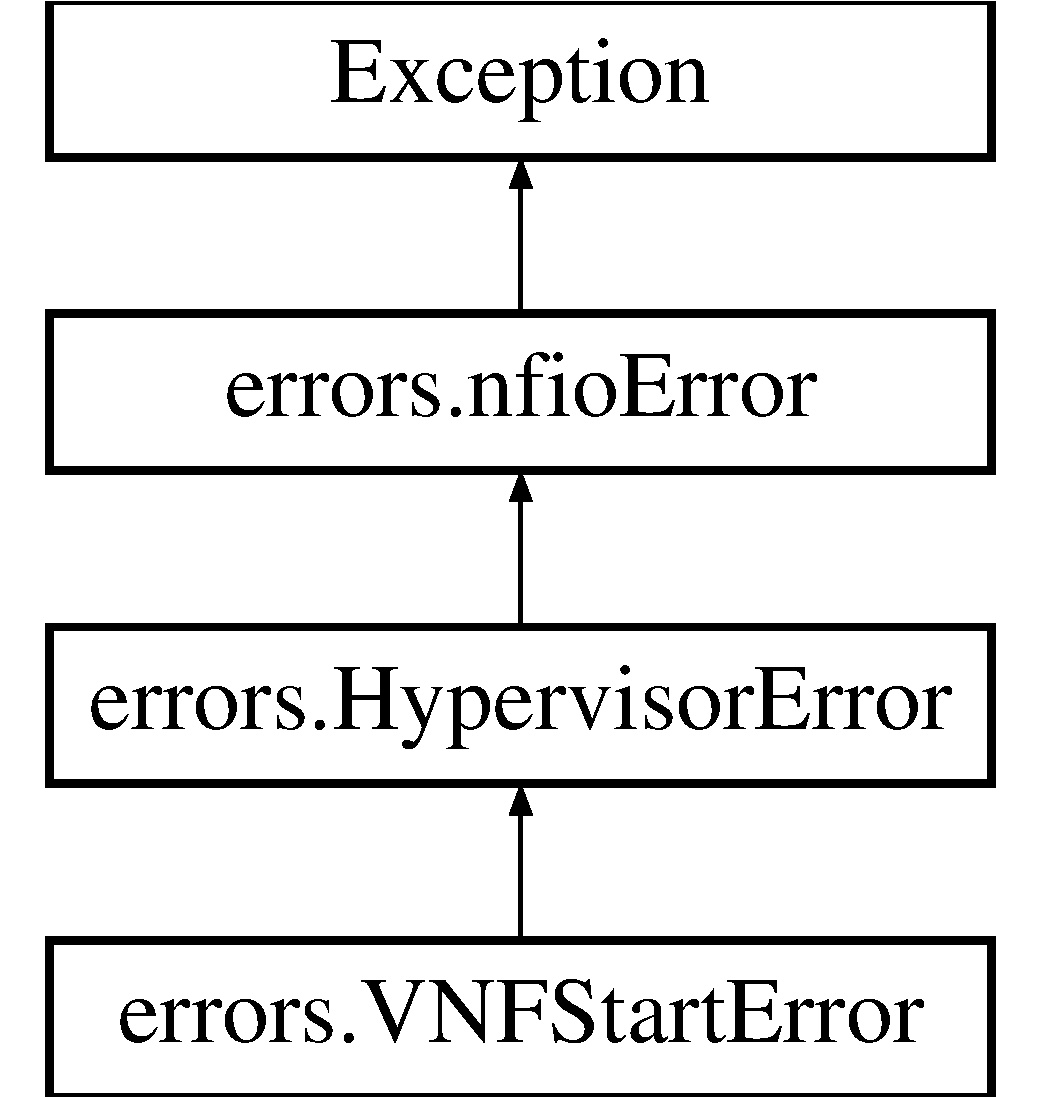
\includegraphics[height=3.000000cm]{classerrors_1_1VNFStartError}
\end{center}
\end{figure}


The documentation for this class was generated from the following file\-:\begin{DoxyCompactItemize}
\item 
/home/nfuser/nf.\-io/src/errors.\-py\end{DoxyCompactItemize}

\hypertarget{classerrors_1_1VNFStopError}{\section{errors.\-V\-N\-F\-Stop\-Error Class Reference}
\label{classerrors_1_1VNFStopError}\index{errors.\-V\-N\-F\-Stop\-Error@{errors.\-V\-N\-F\-Stop\-Error}}
}
Inheritance diagram for errors.\-V\-N\-F\-Stop\-Error\-:\begin{figure}[H]
\begin{center}
\leavevmode
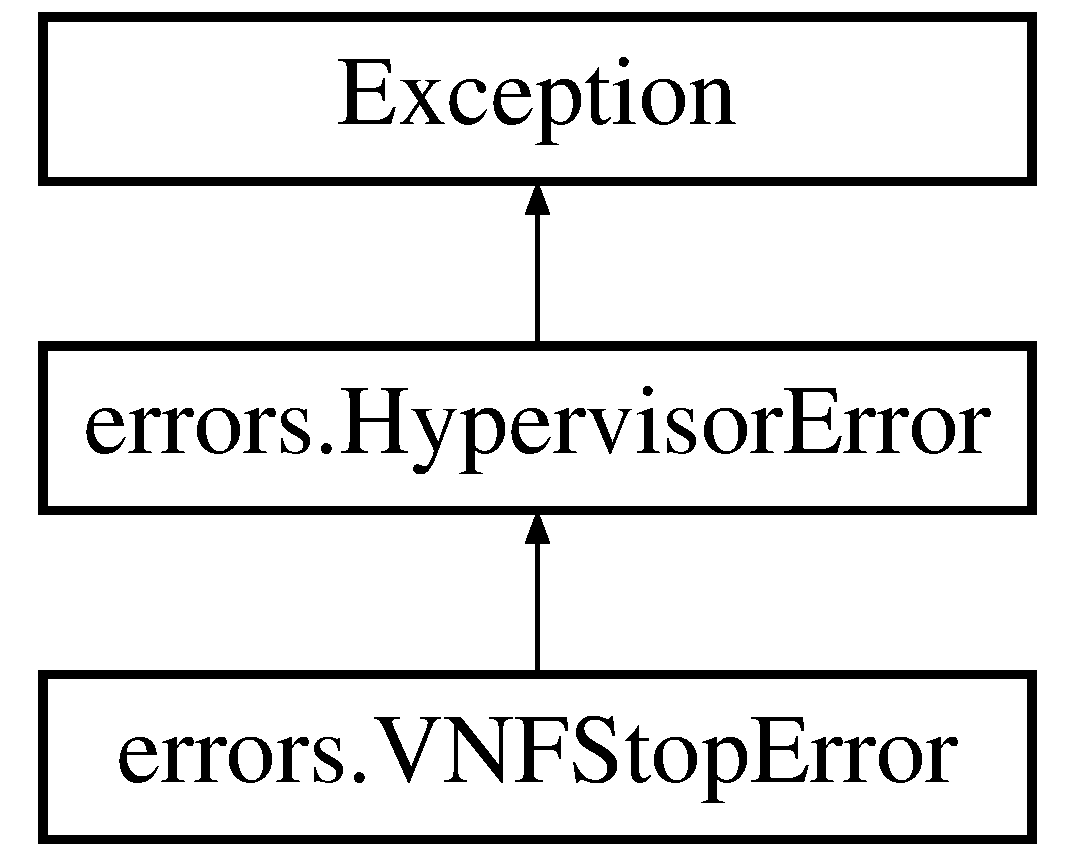
\includegraphics[height=3.000000cm]{classerrors_1_1VNFStopError}
\end{center}
\end{figure}


The documentation for this class was generated from the following file\-:\begin{DoxyCompactItemize}
\item 
/home/nfuser/nf.\-io/src/errors.\-py\end{DoxyCompactItemize}

\hypertarget{classerrors_1_1VNFUnpauseError}{\section{errors.\-V\-N\-F\-Unpause\-Error Class Reference}
\label{classerrors_1_1VNFUnpauseError}\index{errors.\-V\-N\-F\-Unpause\-Error@{errors.\-V\-N\-F\-Unpause\-Error}}
}
Inheritance diagram for errors.\-V\-N\-F\-Unpause\-Error\-:\begin{figure}[H]
\begin{center}
\leavevmode
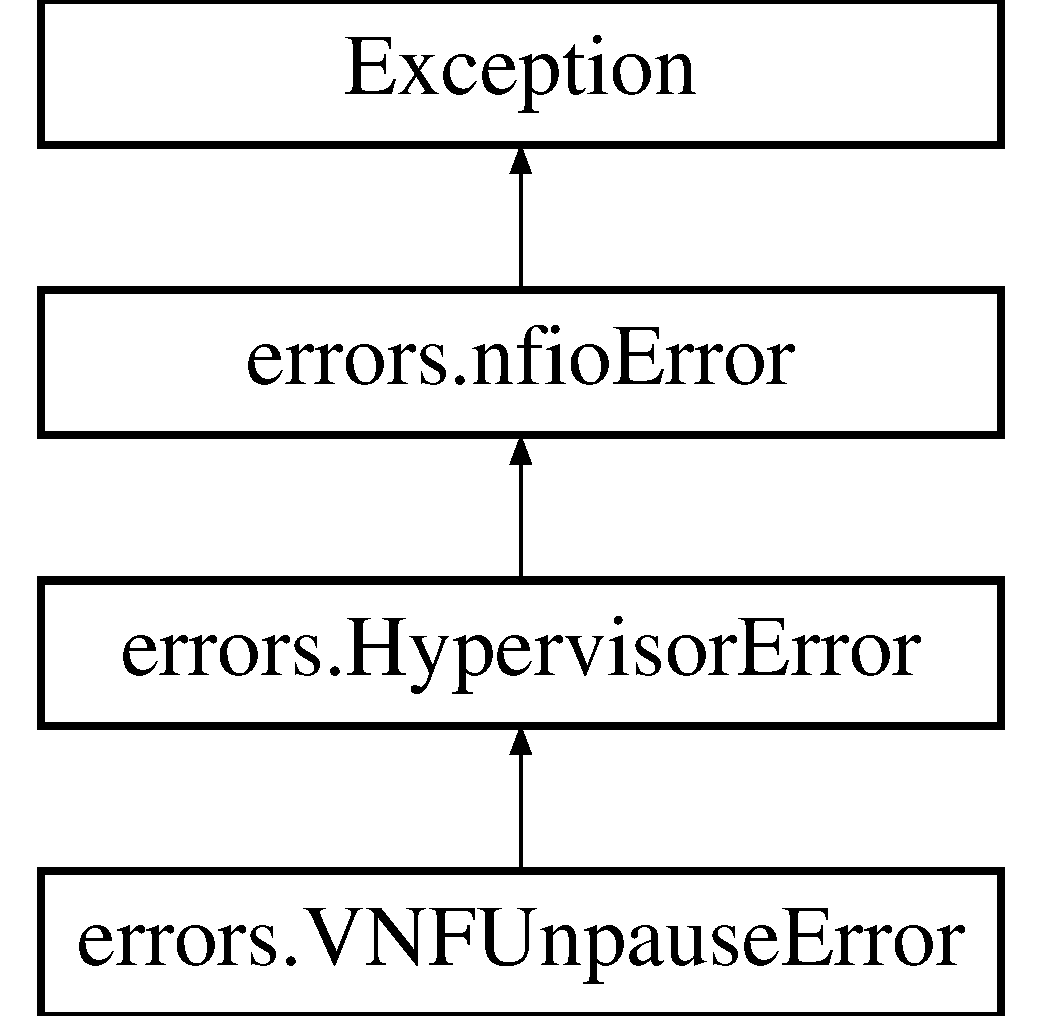
\includegraphics[height=4.000000cm]{classerrors_1_1VNFUnpauseError}
\end{center}
\end{figure}
\subsection*{Public Member Functions}
\begin{DoxyCompactItemize}
\item 
\hypertarget{classerrors_1_1VNFUnpauseError_a85aae2b447871d3ca8a4c9253b0f378b}{def {\bfseries \-\_\-\-\_\-init\-\_\-\-\_\-}}\label{classerrors_1_1VNFUnpauseError_a85aae2b447871d3ca8a4c9253b0f378b}

\end{DoxyCompactItemize}
\subsection*{Public Attributes}
\begin{DoxyCompactItemize}
\item 
\hypertarget{classerrors_1_1VNFUnpauseError_a80bf041b87465d52bde24a08444c0b6b}{{\bfseries errno}}\label{classerrors_1_1VNFUnpauseError_a80bf041b87465d52bde24a08444c0b6b}

\end{DoxyCompactItemize}


\subsection{Detailed Description}


Definition at line 55 of file errors.\-py.



The documentation for this class was generated from the following file\-:\begin{DoxyCompactItemize}
\item 
Wat\-N\-F\-V/nf.\-io/src/errors.\-py\end{DoxyCompactItemize}

%--- End generated contents ---

% Index
\newpage
\phantomsection
\addcontentsline{toc}{chapter}{Index}
\printindex

\end{document}
